\documentclass[a4paper,13pt]{report}
\usepackage[left=3cm,right=2cm,top=2cm,bottom=2cm]{geometry}
\usepackage[utf8]{vietnam}
\usepackage{amsmath,amsxtra,amssymb,latexsym, amscd,amsthm}
\usepackage{indentfirst}
\usepackage{enumerate}
\usepackage{graphicx}
\usepackage{todonotes}
\usepackage{lastpage}
\usepackage{empheq}
% \usepackage[a4paper,margin=1in]{geometry}
\usepackage[unicode]{hyperref}
% \usepackage{biblatex}
\usepackage{titlesec}
\usepackage[vietnamese]{babel}
\usepackage[sorting=none]{biblatex}
\usepackage{fancyhdr}
\fancyhead[R]{\thepage} % thiết lập nội dung mới cho header bên phải

\titleformat{\section}
{\huge\bfseries}{\thesection}{1em}{}
\titleformat{\subsection}{\normalfont\Large\bfseries}{\thesubsection}{1em}{}
\titleformat{\subsubsection}
{\normalfont\Large\bfseries}{\thesubsubsection}{1em}{}
% \titlespacing*{\subsubsection}{0pt}{\baselineskip}{0.5em}
\makeatletter
\newcommand*{\rom}[1]{\expandafter\@slowromancap\romannumeral #1@}
\renewcommand{\thesubsection}{\thesection.\alph{subsection}}
\newcommand{\eqv}{\Leftrightarrow}
\renewcommand\thesection{\Roman{section}}
\renewcommand\thesubsection{\arabic{subsection}}
\hypersetup{
    colorlinks=true,
    linkcolor=black,
    filecolor=magenta,      
    urlcolor=gray,
    pdftitle={BÁO CÁO GIỮA KÌ},
    pdfpagemode=FullScreen,
    }

\usepackage{listings}
\usepackage{color}
\definecolor{dkgreen}{rgb}{0,0.6,0}
\definecolor{gray}{rgb}{0.5,0.5,0.5}
\definecolor{mauve}{rgb}{0.58,0,0.82}

\lstset{frame=tb,
  language=Java,
  aboveskip=3mm,
  belowskip=3mm,
  showstringspaces=false,
  columns=flexible,
  basicstyle={\small\ttfamily},
  numbers=none,
  numberstyle=\tiny\color{gray},
  keywordstyle=\color{blue},
  commentstyle=\color{dkgreen},
  stringstyle=\color{mauve},
  breaklines=true,
  breakatwhitespace=true,
  tabsize=3
}
\usepackage{tocloft}
\usepackage{enumitem}
\usepackage{fancyhdr}
% \AtBeginDocument{\settowidth{\sectionnumwidth}{VIII.\ }}
\begin{document}

\setlength{\parindent}{0.87cm}
\setlist[itemize]{labelsep=1em}
\setlength{\cftsecnumwidth}{3.7em} %3.2
% \setlength{\cftsubsecnumwidth}{\cftsecnumwidth}
\setlength{\cftsubsecindent}{3.7em}
\setlength{\cftsubsubsecindent}{6.05em}
% \setlength{\cftsecindent}{-1.75em} %-1.75
\fontsize{14pt}{18pt}\selectfont % Lệnh thay đổi cỡ chữ thành cỡ 13, cỡ dòng 18 (theo quy chuẩn của Khóa Luận TN).

\titleformat{\paragraph}
{\normalfont\normalsize\bfseries}{\theparagraph}{1em}{}
\titlespacing*{\paragraph}
{0pt}{3.25ex plus 2ex minus .2ex}{1.5ex plus .2ex}

% \setlength{\baselineskip}{18truept}

\begin{center}

{\large\bf ĐẠI HỌC QUỐC GIA HÀ NỘI \\ 
TRƯỜNG ĐẠI HỌC CÔNG NGHỆ}\\

% {\large\bf KHOA CÔNG NGHỆ THÔNG TIN} \\

{————————————————–}

% \vskip 3cm
% {\bf KHÓA LUẬN TỐT NGHIỆP}\\[1cm]

\vskip 2.5cm
\begin{center}
    
\includegraphics[width=0.35\linewidth]{figure/uet.jpg}
\end{center}
\vskip 2.5cm
{\huge\bf \textbf{BÁO CÁO GIỮA KÌ}}\\

\vskip 1cm

{\LARGE\bf \textbf{Bộ môn: An toàn an ninh mạng}}\\

\vskip 2.5cm
% \includegraphics[scale = 0.15]{UET.jpg}
%  \vskip 1cm

\begin{tabular}{r l r}

Giảng viên hướng dẫn:&{\bf TS. Nguyễn Đại Thọ}\\[0.5cm]

Người thực hiện:  &{\bf Nguyễn Trung Hiếu}\\[0.5cm]

Mã sinh viên: & {\bf 21020017}\\[0.5cm]

\end{tabular}

\vskip 3.5cm

{\bf HÀ NỘI, 07/2023}

\end{center}


% \title{Selenium}

% \maketitle
% \newpage
% \newpage

\tableofcontents
% \thispagestyle{empty}
% \setcounter{arabic}{3}
% \pagestyle{plain}
% \pagenumbering{gobble}

\newpage

\listoffigures

\newpage

\section{Installing Certificate Services}
\subsection{Activities}

\noindent {\bf{Bước 1:}} Truy cập vào đường dẫn \href{https://www.microsoft.com/en-us/evalcenter/evaluate-windows-server-2016}{Link} để download file ISO. Sau đó, chọn {\bf Download the ISO}.

\begin{figure}[!htb]
    \centering
    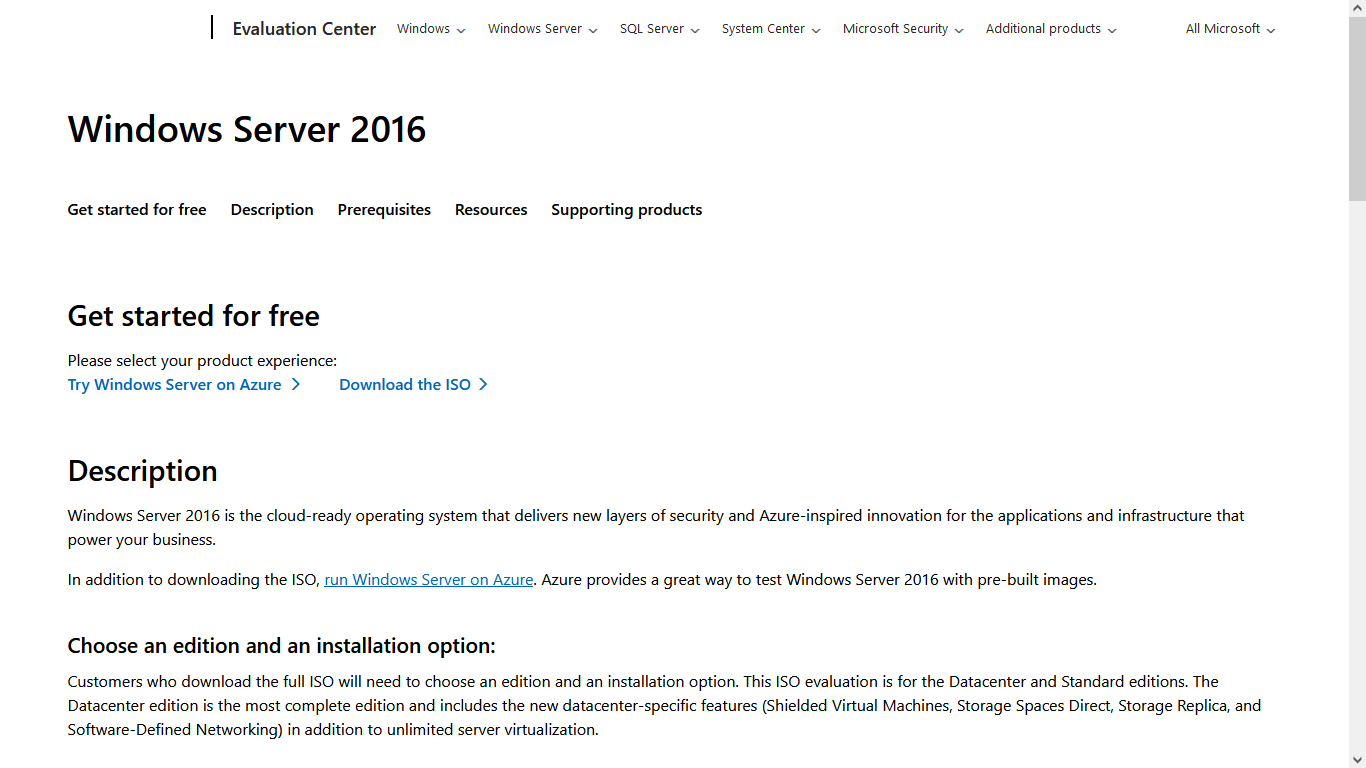
\includegraphics[width=1\linewidth]{figure//chapter4//lab4_1/download_iso.png}
    \caption{Màn hình tải file ISO}
    \label{fig:enter-label}
\end{figure}

\noindent {\bf{Bước 2:}} Điền các thông tin cần thiết rồi chọn {\bf Download}.

\begin{figure}[!htb]
    \centering
    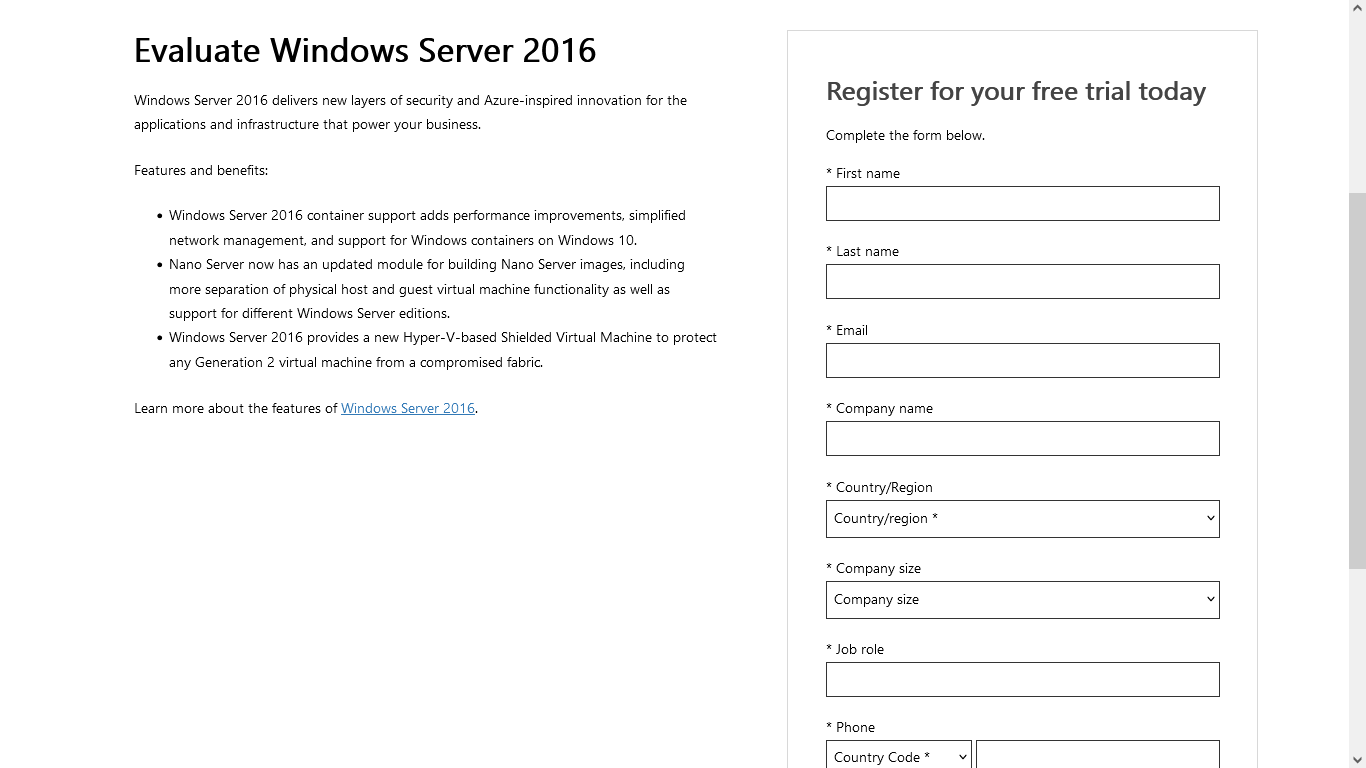
\includegraphics[width=1\linewidth]{figure//chapter4//lab4_1/input_info.png}
    \caption{Nhập thông tin cá nhân}
    \label{fig:enter-label}
\end{figure}

\noindent Sau đó chọn phiên bản phù hợp rồi lưu vào máy.

\vskip 0.5cm
\noindent {\bf{Bước 3:}} Tải VirtualBox và tạo ra một máy ảo Windows bằng file ISO vừa tải. Chọn Microsoft Windows và Windows 2016. Khởi động máy ảo.

\begin{figure}[!htb]
    \centering
    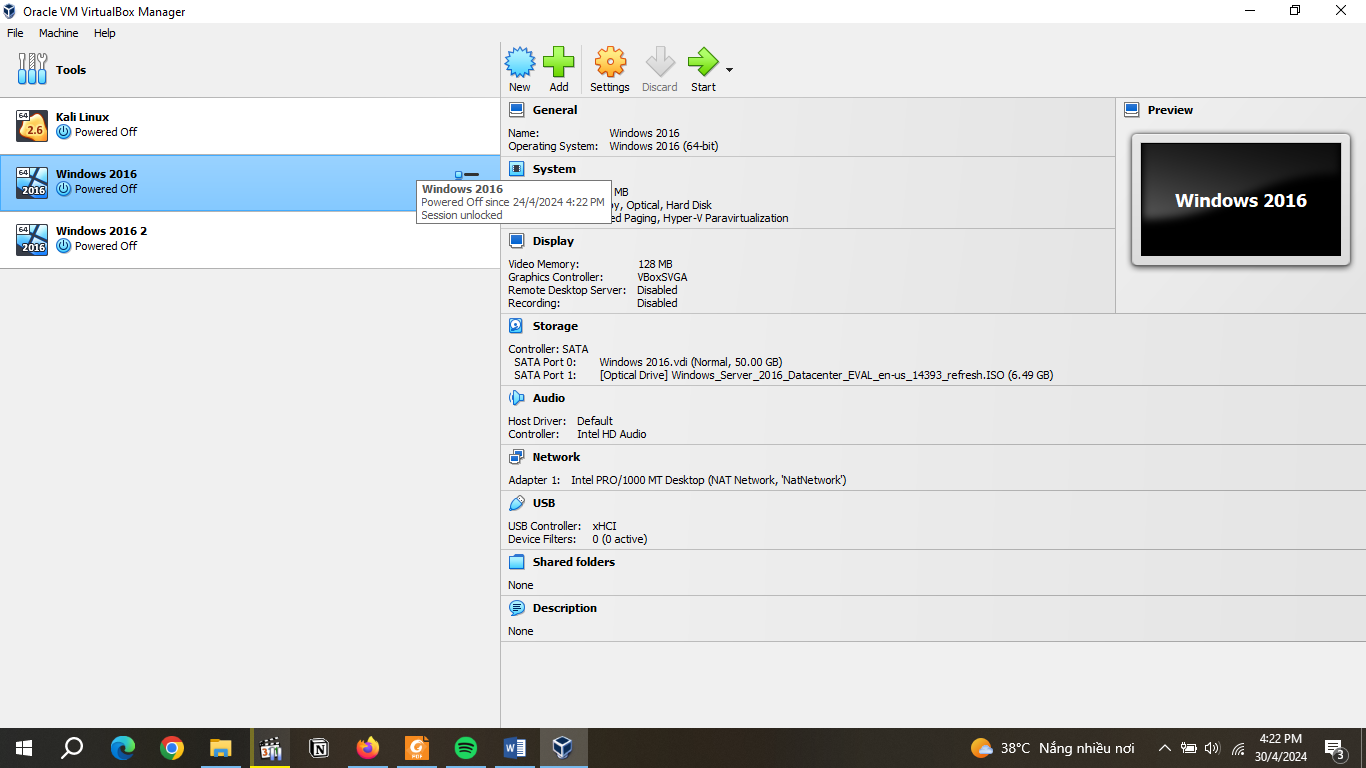
\includegraphics[width=1\linewidth]{figure//chapter4//lab4_1/start_vm.png}
    \caption{Khởi động máy ảo Windows 2016}
    \label{fig:enter-label}
\end{figure}

\vskip 0.5cm
\noindent {\bf{Bước 4:}} Chọn ngôn ngữ, thời gian và bàn phím phù hợp. Nhấn {\bf Install Now} để tiến hành cài đặt. Tại phần chọn Windows Setup, chọn {\bf Windows Server 2016 Standard Evaluation (Desktop Experience)}.

\begin{figure}[!htb]
    \centering
    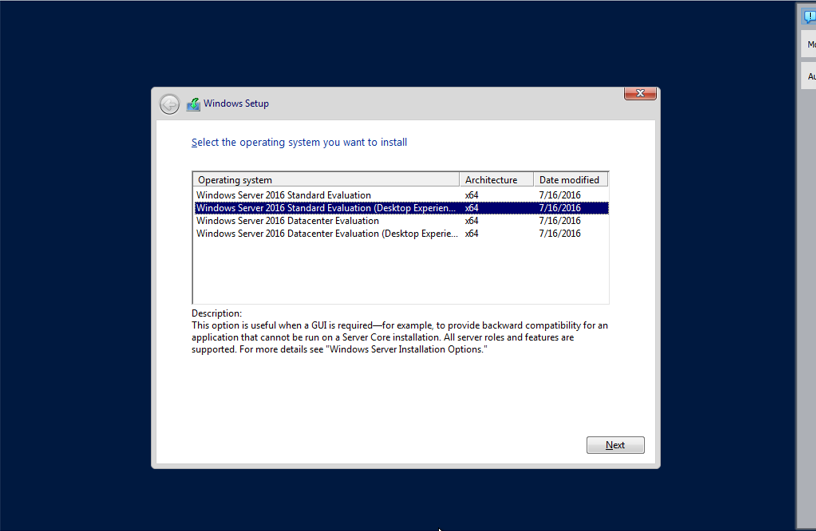
\includegraphics[width=0.8\linewidth]{figure//chapter4//lab4_1/select_os.png}
    \caption{Chọn hệ điều hành}
    \label{fig:enter-label}
\end{figure}

\vskip 0.5cm

\newpage

\noindent {\bf{Bước 5:}} Chọn {\bf Custom: Install Windows only (advanced)}. 

\begin{figure}[!htb]
    \centering
    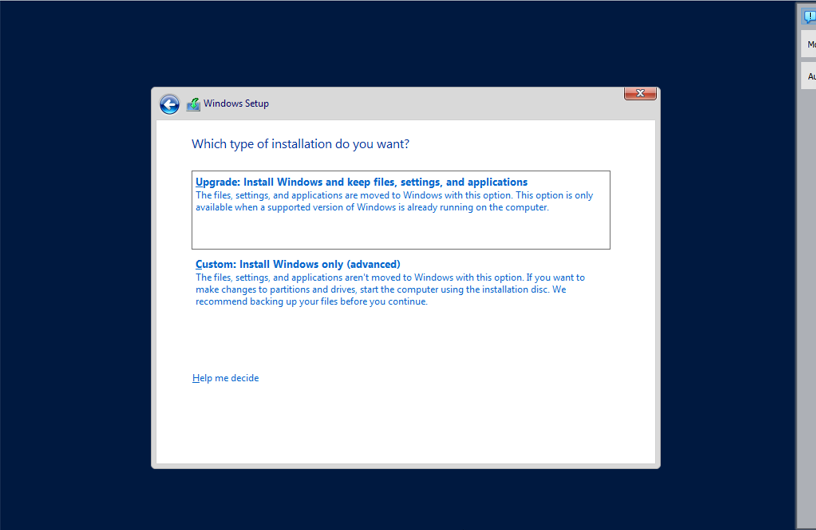
\includegraphics[width=1\linewidth]{figure//chapter4//lab4_1/select_setup_type.png}
    \caption{Chọn cách cài đặt}
    \label{fig:enter-label}
\end{figure}

\noindent {\bf{Bước 6:}} Tiếp tục chọn Next và cài đặt mật khẩu cho Administrator là {\bf Pa\$\$word}. Sau đó đăng nhập vào hệ thống với tài khoản Administrator.

\begin{figure}[!htb]
    \centering
    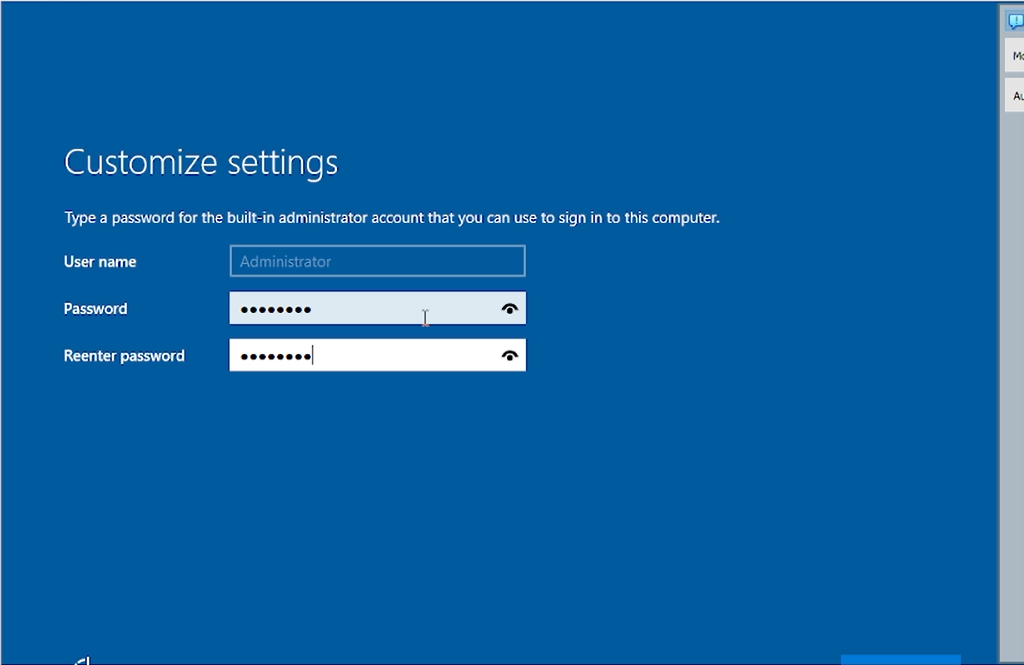
\includegraphics[width=1\linewidth]{figure//chapter4//lab4_1/enter_password.png}
    \caption{Enter Caption}
    \label{fig:enter-label}
\end{figure}

\noindent {\bf{Bước 7:}} Mở Server Manager, chọn \textbf{Manage} rồi chọn \textbf{Add Roles and Features}. Click \textbf{Next} cho tới khi thấy màn hình \textbf{Server Roles}.

\begin{figure}[!htb]
    \centering
    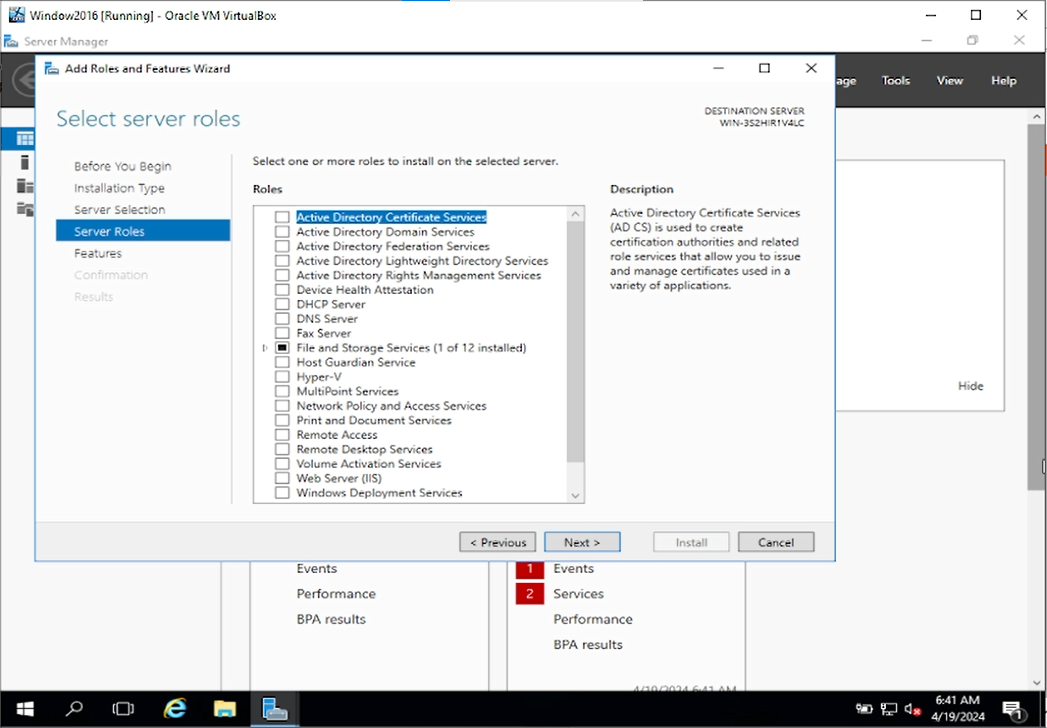
\includegraphics[width=0.9\linewidth]{figure//chapter4//lab4_1/select_add_roles_and_features.png}
    \caption{Màn hình Server Roles}
    \label{fig:enter-label}
\end{figure}

% \newpage

\noindent {\bf{Bước 8:}} Chọn \textbf{Active Directory Domain Services}. Sau đó chọn \textbf{Add Feature} ở màn hình hiện lên. Tiếp theo nhấn \textbf{Next} liên tục rồi \textbf{Install}.

\begin{figure}[!htb]
    \centering
    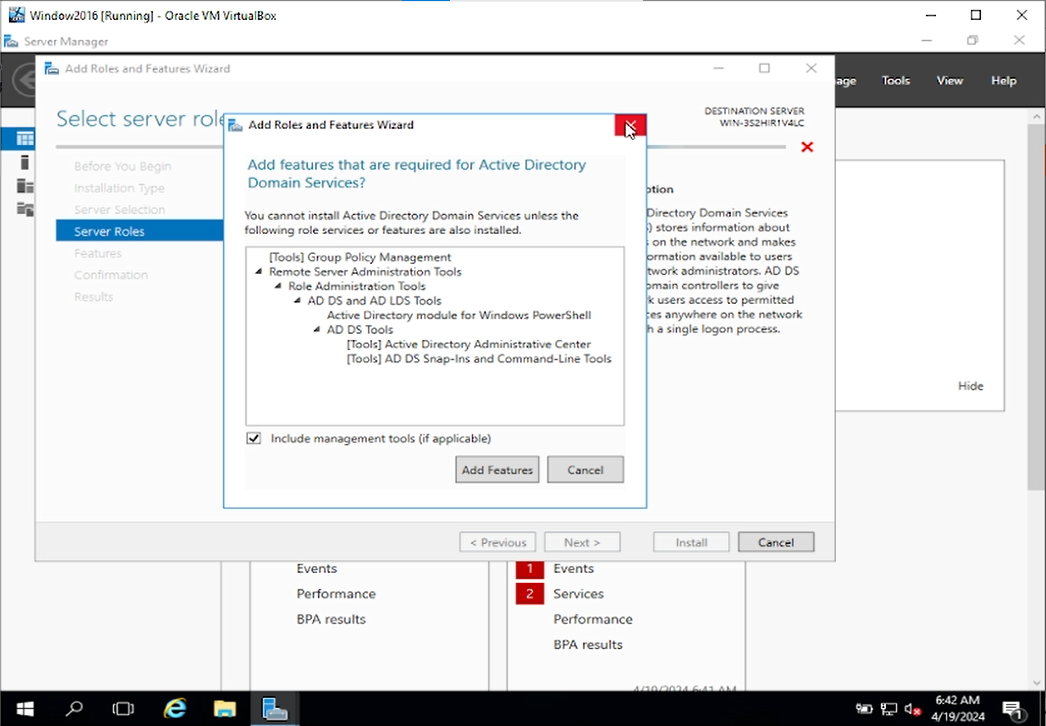
\includegraphics[width=0.9\linewidth]{figure//chapter4//lab4_1/add_feature.png}
    \caption{Màn hình Add Features}
    \label{fig:enter-label}
\end{figure}

\noindent {\bf{Bước 9:}} Chọn vào cờ thông báo ở phía trên màn hình và chọn \textbf{Promote this server to a domain controller}.

\begin{figure}[!htb]
    \centering
    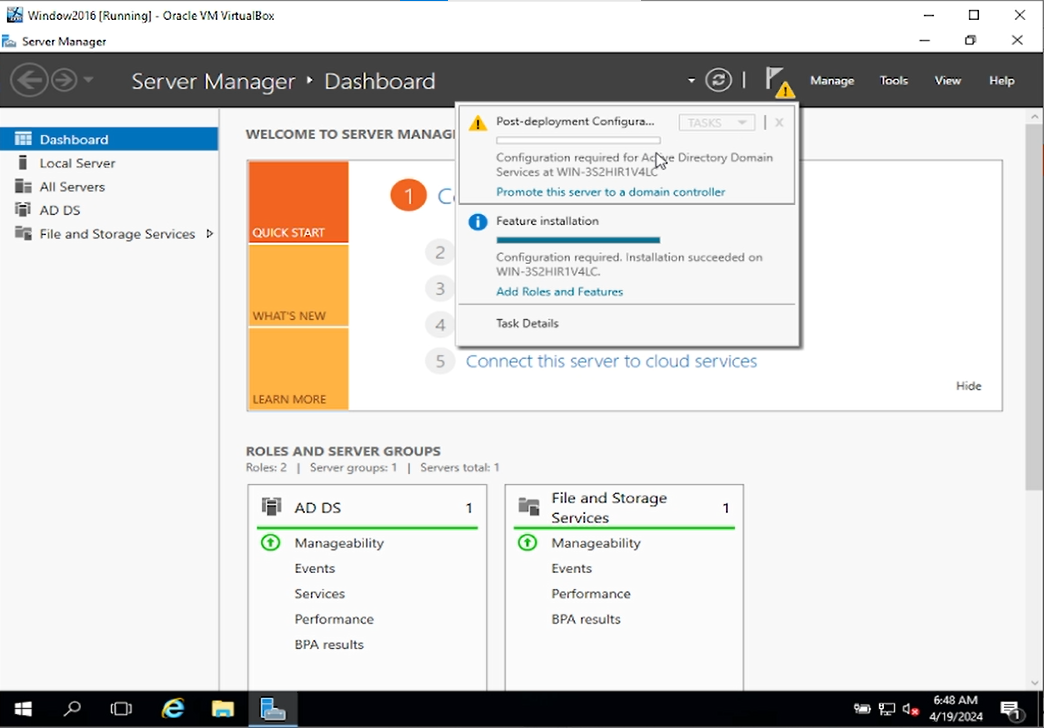
\includegraphics[width=0.9\linewidth]{figure//chapter4//lab4_1/promote_server.png}
    \caption{Chọn cờ thông báo}
    \label{fig:enter-label}
\end{figure}

\noindent {\bf{Bước 10:}} Chọn \textbf{Add a new forest} và điền \textbf{Test.local} vào phần \textbf{Root domain name}.

\begin{figure}[!htb]
    \centering
    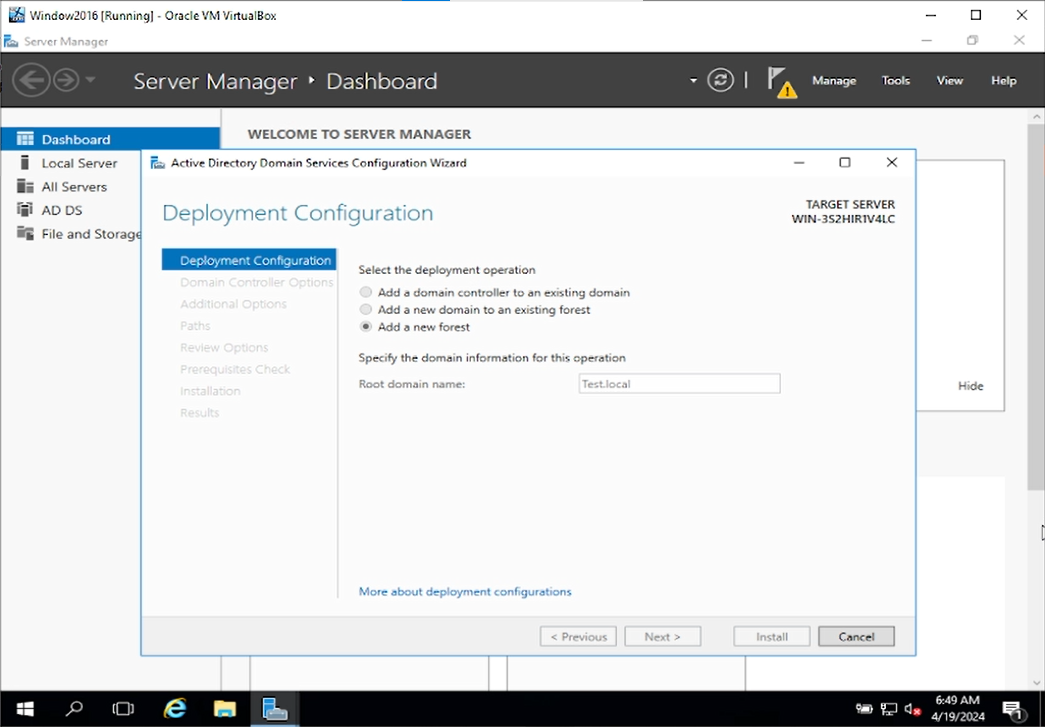
\includegraphics[width=0.9\linewidth]{figure//chapter4//lab4_1/test_local.png}
    \caption{Add a new forest}
    \label{fig:enter-label}
\end{figure}

\noindent {\bf{Bước 11:}} Điền mật khẩu là \textbf{Pa\$\$word}, rồi chọn \textbf{Next} hai lần.

\begin{figure}[!htb]
    \centering
    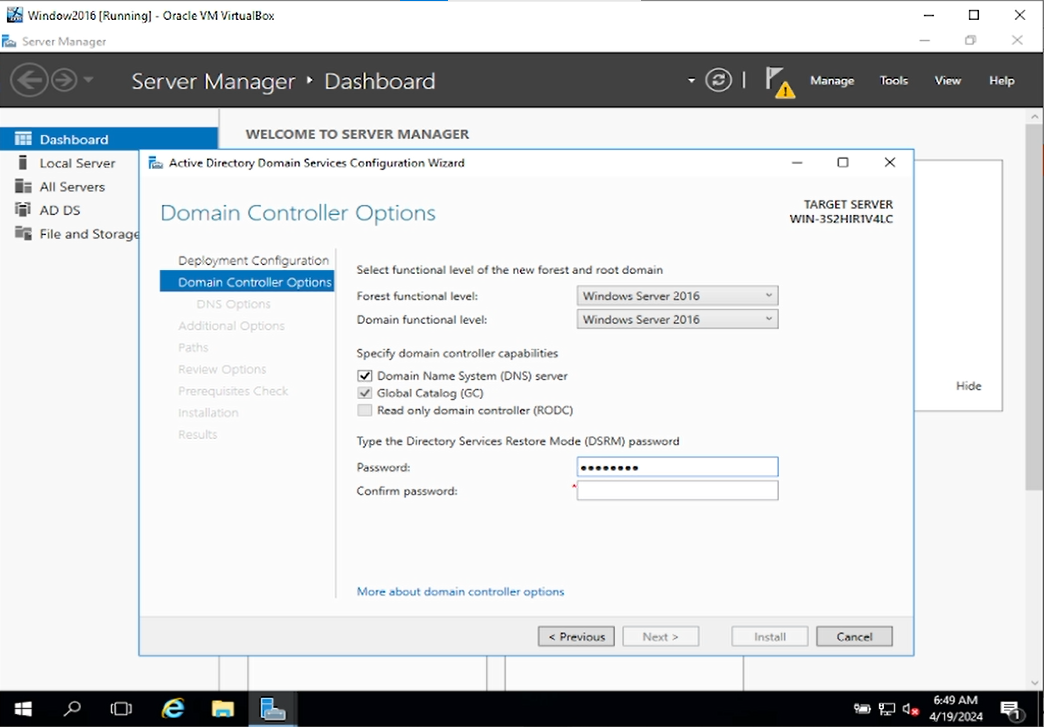
\includegraphics[width=0.9\linewidth]{figure//chapter4//lab4_1/enter_password_2.png}
    \caption{Nhập DSMR Password}
    \label{fig:enter-label}
\end{figure}

\noindent {\bf{Bước 11:}} Nhập \textbf{TEST} cho phần NetBIOS domain name và chọn \textbf{Next} ba lần.

\begin{figure}[!htb]
    \centering
    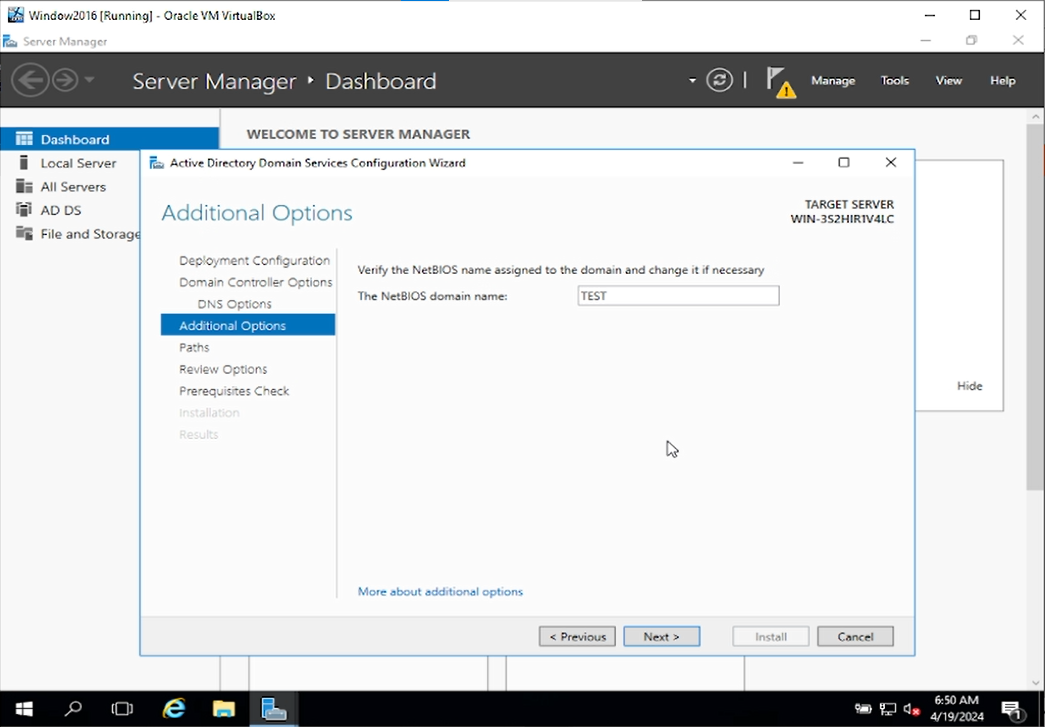
\includegraphics[width=0.9\linewidth]{figure//chapter4//lab4_1/enter_netbios_domain_name.png}
    \caption{Nhập NetBIOS domain name}
    \label{fig:enter-label}
\end{figure}

\noindent Tiếp tục chọn \textbf{Next} và cuối cùng chọn \textbf{Install}.

\noindent {\bf{Bước 12:}} Lặp lại quá trình cho tới khi gặp phải màn hình Server Roles. Tại đây, chọn \textbf{Active Directory Certificate Services}. Chọn \textbf{Add Features}.

\begin{figure}[!htb]
    \centering
    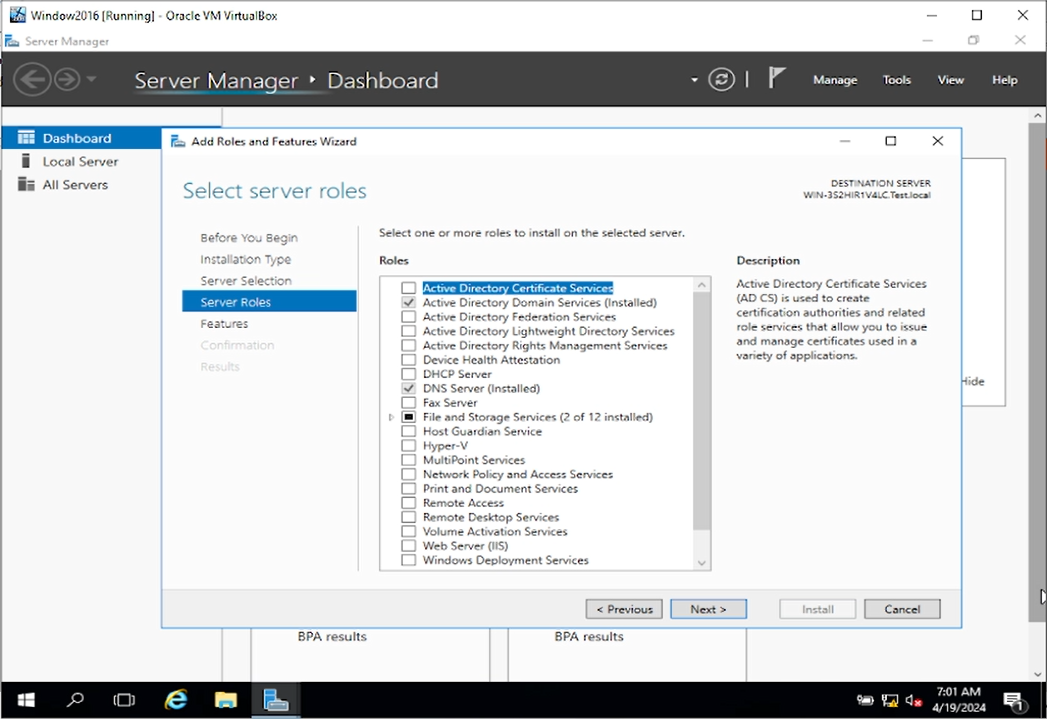
\includegraphics[width=0.9\linewidth]{figure//chapter4//lab4_1/add_active_domain_certificate_services.png}
    \caption{Chọn Active Directory Certificate Servicies}
    \label{fig:enter-label}
\end{figure}

\noindent {\bf{Bước 13:}} Cứ thế tiếp tục cho tới màn hình \textbf{AD CS} và\textbf{Role Services}. Chọn \textbf{Certification Authority} và \textbf{Certification Authority Web Enrollment}.

\begin{figure}[!htb]
    \centering
    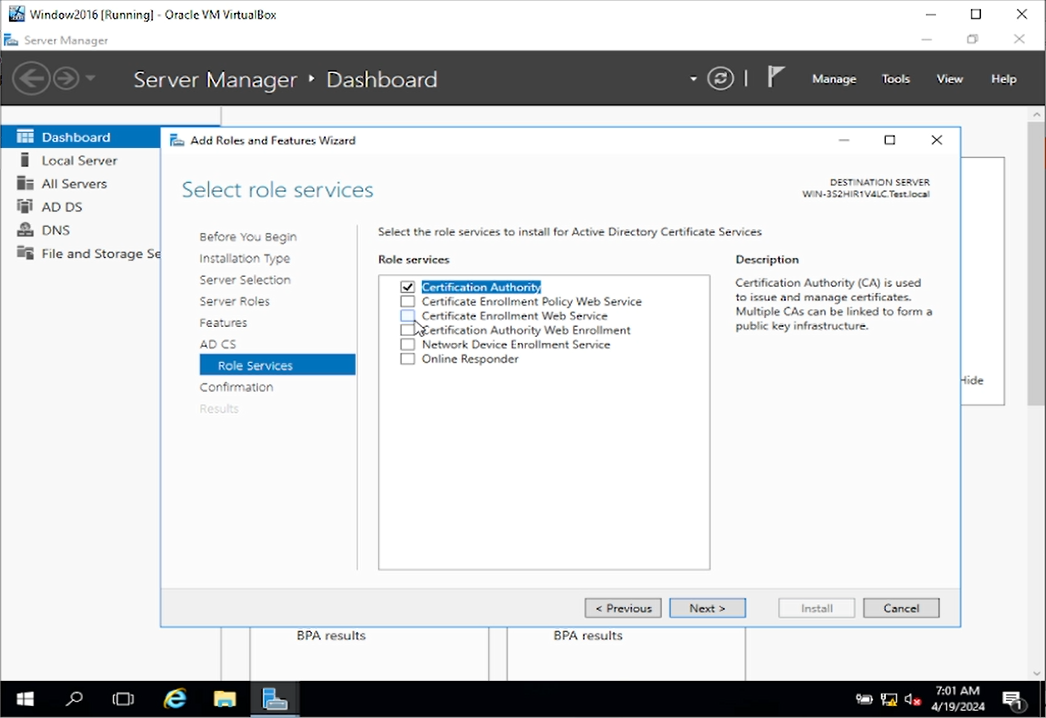
\includegraphics[width=0.9\linewidth]{figure//chapter4//lab4_1/role_service.png}
    \caption{Màn hình Role Services}
    \label{fig:enter-label}
\end{figure}

\noindent Chọn \textbf{Add Feature}, chọn \textbf{Next} và cuối cùng là \textbf{Install}.

\noindent {\bf{Bước 14:}} Vào cờ thông báo, chọn \textbf{Configure Active Directory Certificate Services on the destination server}. 

\begin{figure}[!htb]
    \centering
    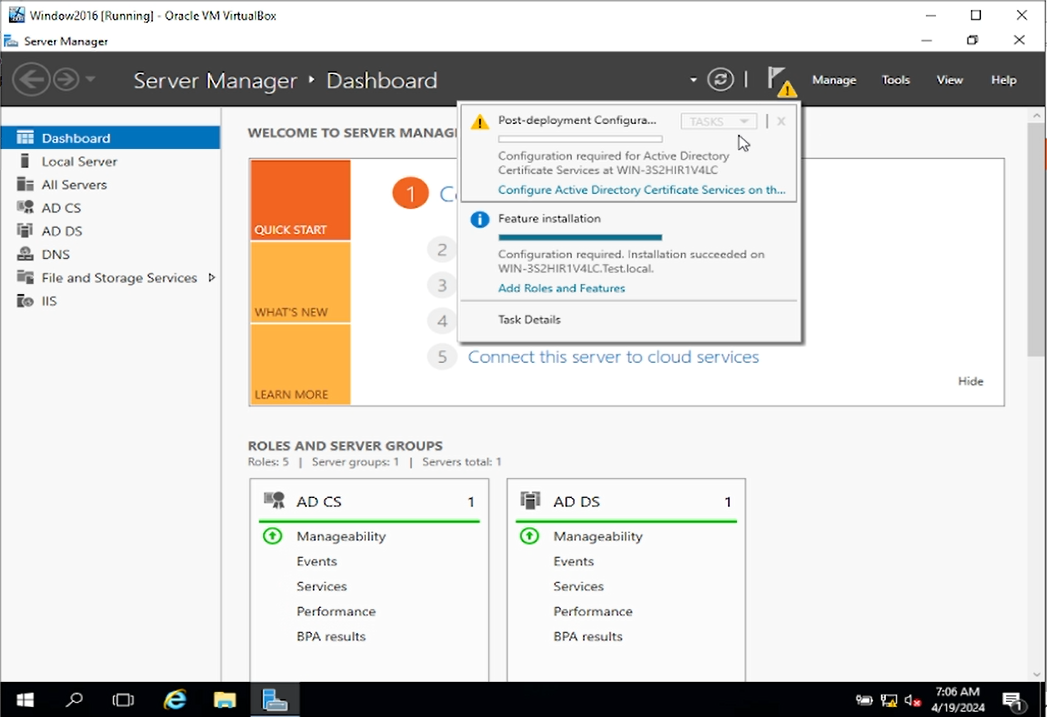
\includegraphics[width=0.9\linewidth]{figure//chapter4//lab4_1/configure_active_directory.png}
    \caption{Màn hình chọn cờ thông báo}
    \label{fig:enter-label}
\end{figure}

\noindent Chọn \textbf{Next} ở màn hình Credentials, chọn \textbf{Certification Authority} và \textbf{Certification Authority Web Enrollment}.

\begin{figure}[!htb]
    \centering
    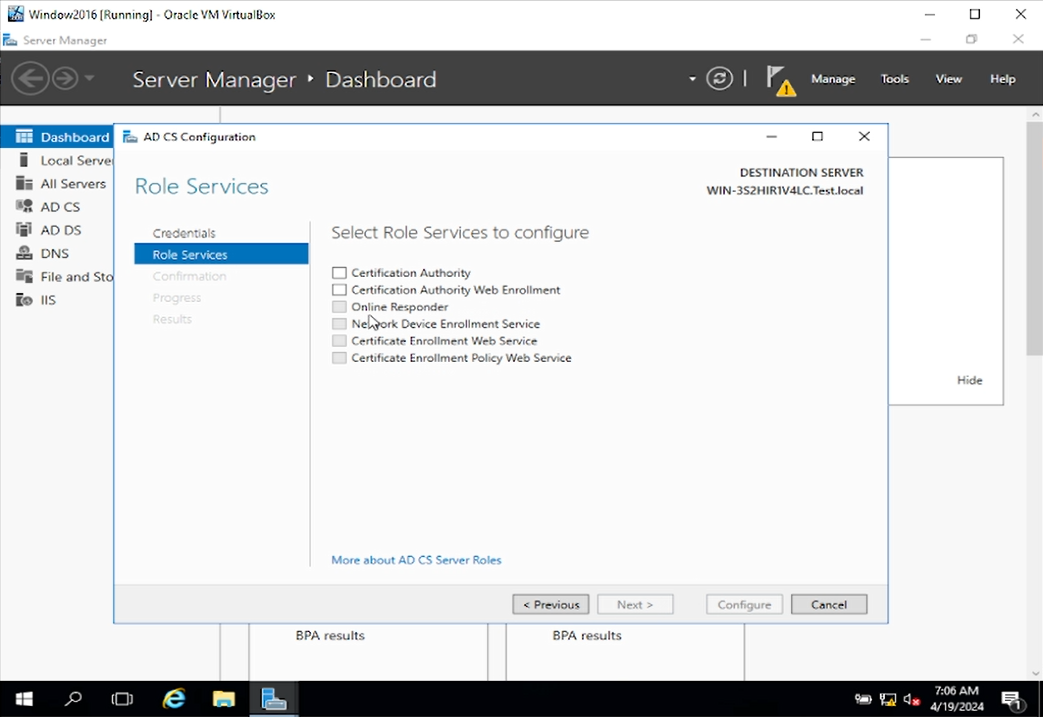
\includegraphics[width=0.85\linewidth]{figure//chapter4//lab4_1/configure_service.png}
    \caption{Chọn Service cần cấu hình}
    \label{fig:enter-label}
\end{figure}

\noindent {\bf{Bước 15:}} Trong các cửa sổ sau đó, sử dụng các lựa chọn đã được chọn mặc định và chọn \textbf{Next}. Cuối cùng chọn \textbf{Configure}.

\begin{figure}[!htb]
    \centering
    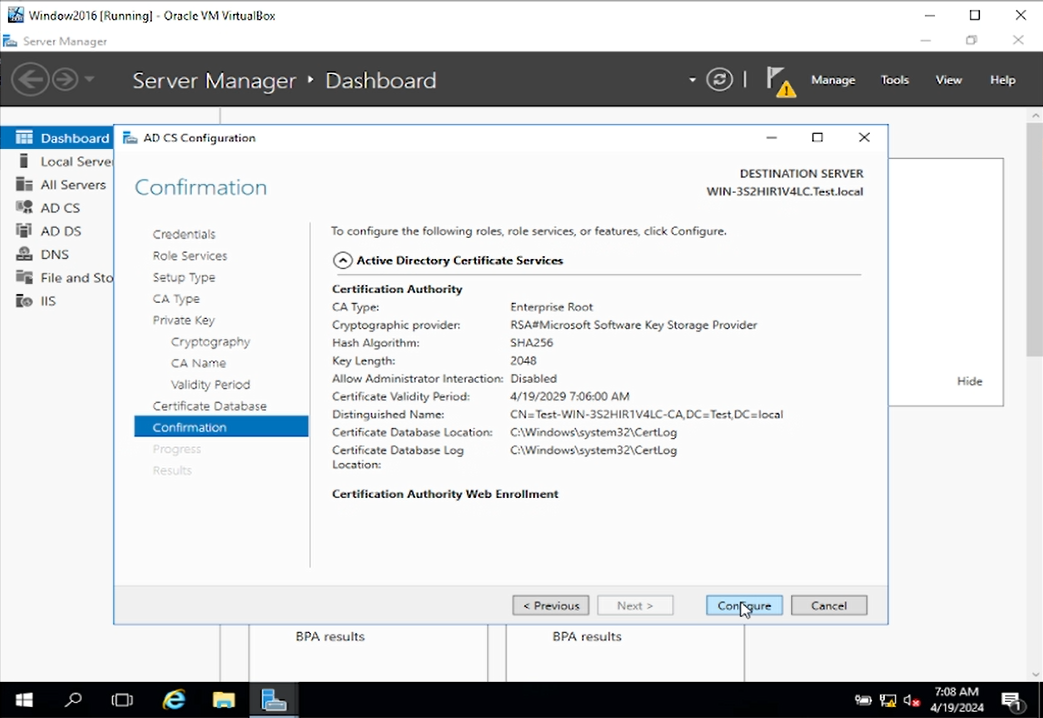
\includegraphics[width=0.9\linewidth]{figure//chapter4//lab4_1/configure_window.png}
    \caption{Màn hình cấu hình AD CS}
    \label{fig:enter-label}
\end{figure}

\noindent {\bf{Bước 16:}} Sau khi cài đặt xong, vào \textbf{Search Windows} và nhập mmc.

\begin{figure}[!htb]
    \centering
    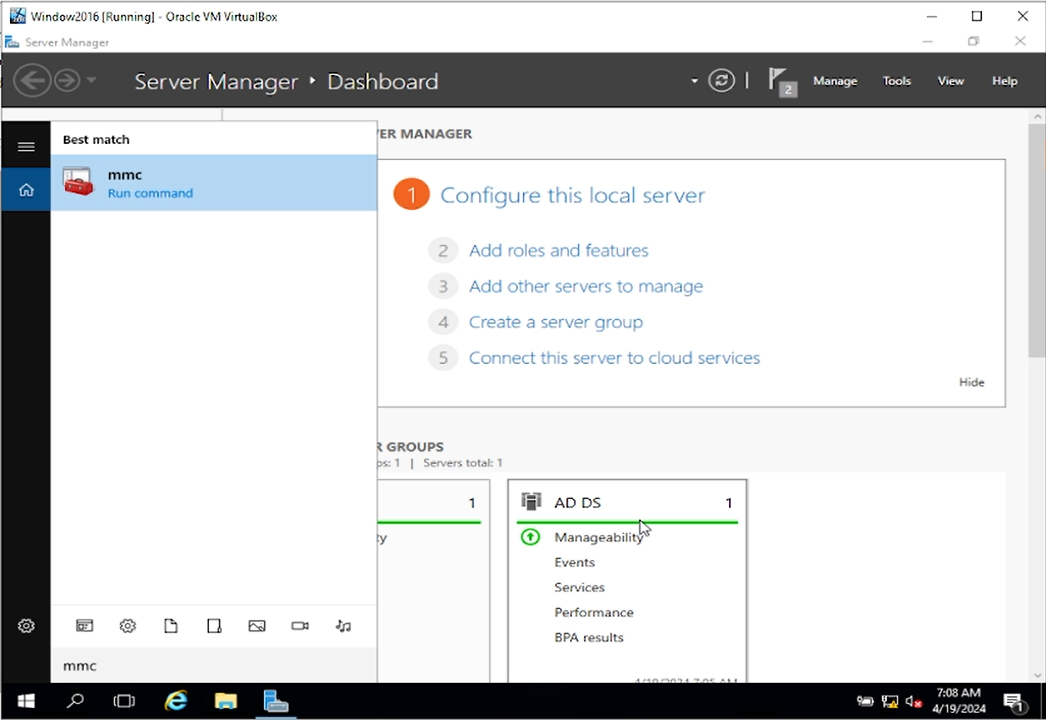
\includegraphics[width=0.9\linewidth]{figure//chapter4//lab4_1/mmc.png}
    \caption{Chọn mmc}
    \label{fig:enter-label}
\end{figure}

\newpage

\noindent {\bf{Bước 17:}} Chọn \textbf{File}, chọn \textbf{Add/Remove Snap-ins}. Sau đó, thêm \textbf{Add Certificate Templates}, \textbf{Certification Authority (Local), Enterprise PKI} và \textbf{Internet Information Service (IIS) Manager}.

\begin{figure}[!htb]
    \centering
    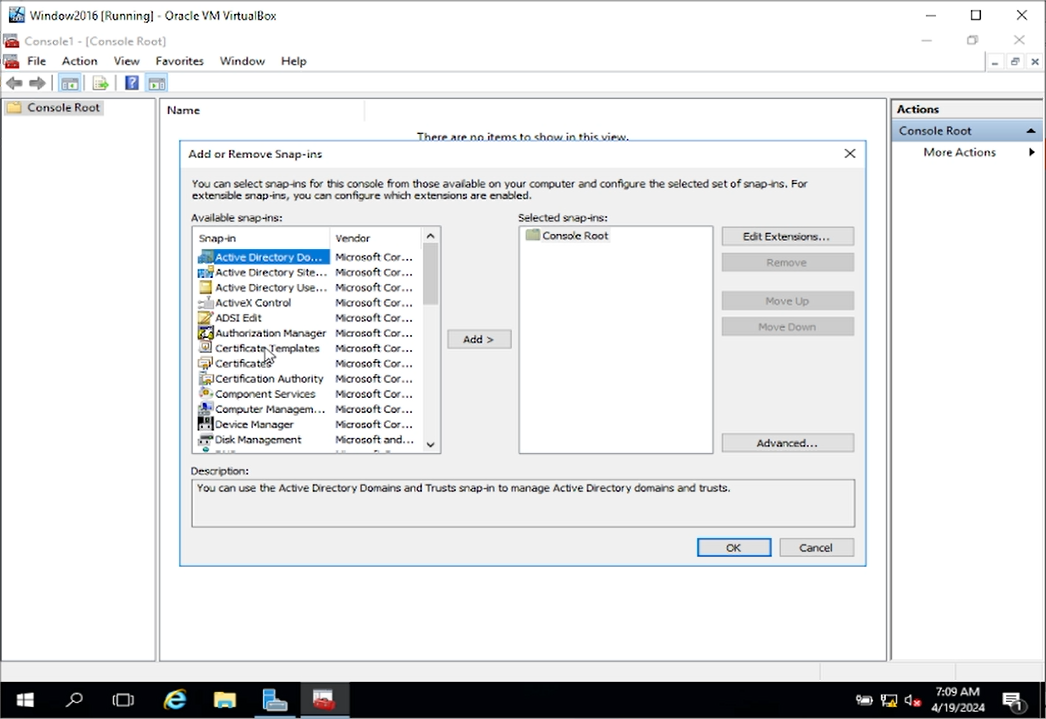
\includegraphics[width=0.9\linewidth]{figure//chapter4//lab4_1/add_snap_in.png}
    \caption{Thêm Snap-ins}
    \label{fig:enter-label}
\end{figure}

\noindent Kết quả nhận được như sau.

\begin{figure}[!htb]
    \centering
    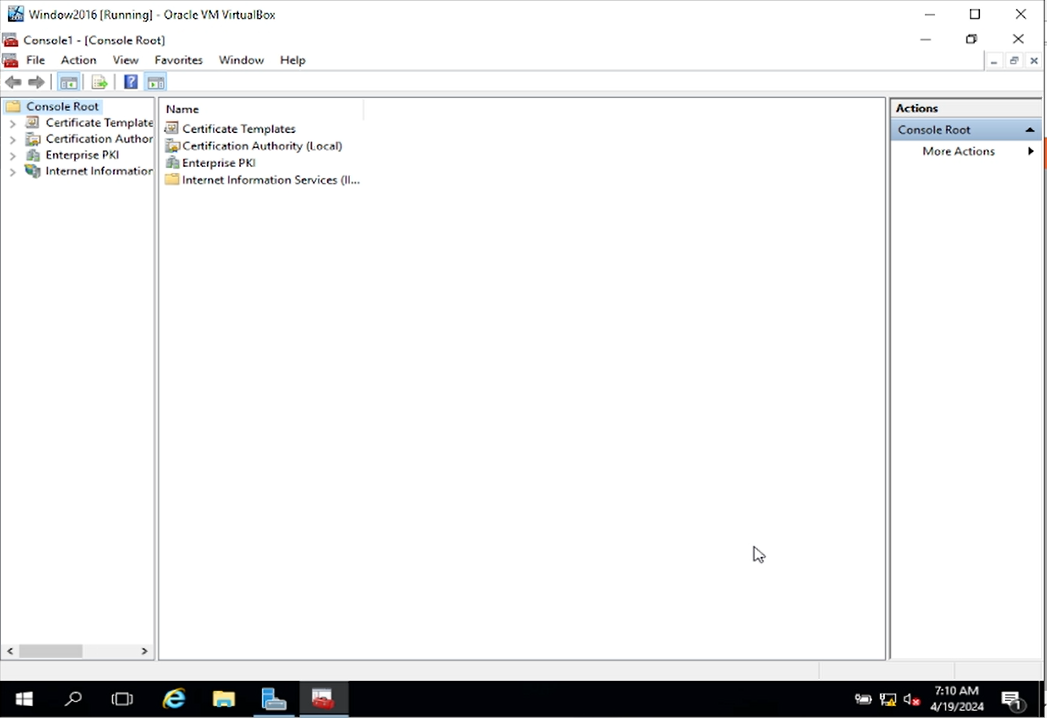
\includegraphics[width=0.9\linewidth]{figure//chapter4//lab4_1/result.png}
    \caption{Kết quả màn hình mmc}
    \label{fig:enter-label}
\end{figure}

\subsection{Review Questions}

\noindent \textbf{Câu 1:} 

B: Active Directory Domain Services.

\noindent \textbf{Câu 2:} 

B: Online Responder.

C: World Wide Web Publishing Service.

D: Network Device Enrollment Service.

\noindent \textbf{Câu 3:} 

C: Enhance certificate revocation checking by setting up an online responder.

\noindent \textbf{Câu 4:} True.

\noindent \textbf{Câu 5:} 


D: A stand-alone CA is integrated with Active Directory Domain Services.
\newpage
\section{Configuring Secure Sockets Layer}
\subsection{Activities}
\noindent {\bf{Bước 1:}} Khởi động lại máy ảo Windows được tạo từ phần 1. 

\noindent {\bf{Bước 2:}} Mở file PKI được lưu từ phần 1. Tại đây, mở rộng phần \textbf{Enterprise PKI} rồi click vào ServerName (bắt đầu bởi Test). Tại đây, có thể nhấn vào CA Certificate để biết thêm chi tiết về certificate này.

\begin{figure}[!htb]
    \centering
    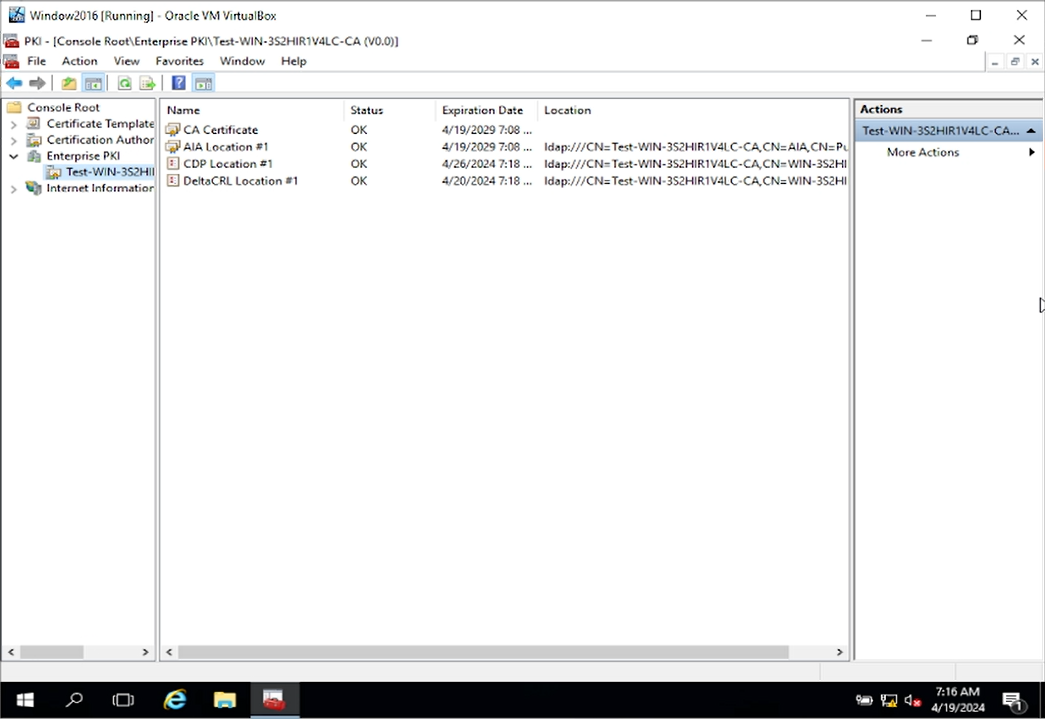
\includegraphics[width=0.8\linewidth]{figure//chapter4//lab4_1/ca_cert.png}
    \caption{Màn hình thông tin trong Enterprise PKI}
    \label{fig:enter-label}
\end{figure}

\begin{figure}[!htb]
    \centering
    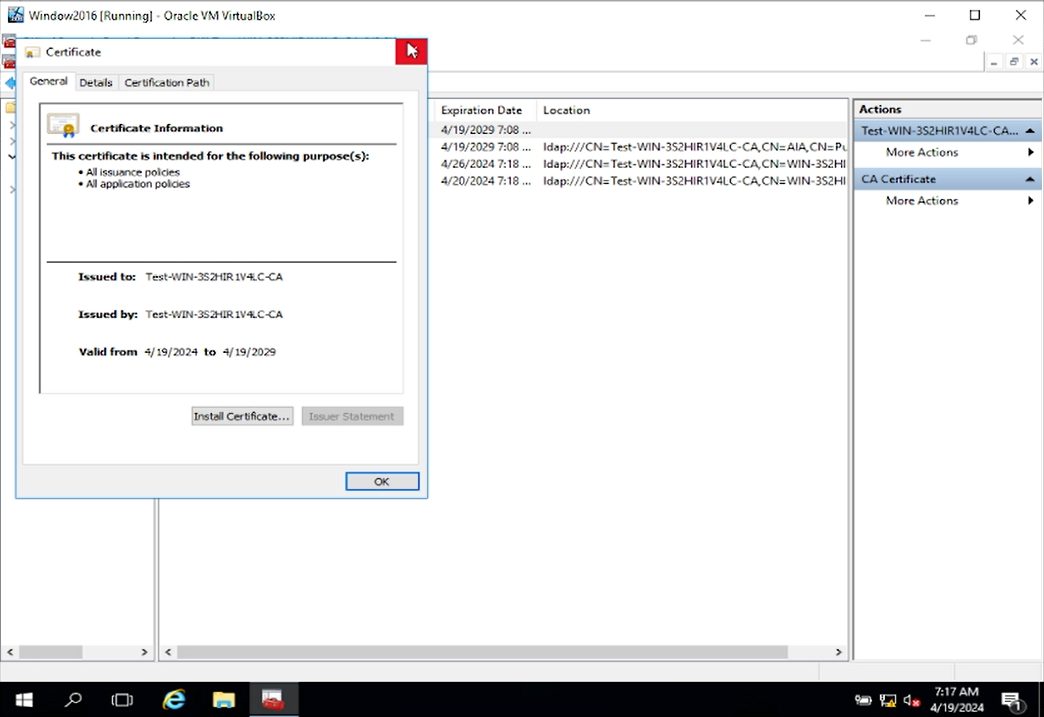
\includegraphics[width=0.8\linewidth]{figure//chapter4//lab4_2/ca_cert_info.png}
    \caption{Thông tin của CA Certificate}
    \label{fig:enter-label}
\end{figure}

\newpage
\noindent {\bf{Bước 3:}} Mở rộng phần \textbf{Certification Authority (Local)} và chọn ServerName. Sau đó chọn các certificate và các mục khác để biết thêm thông tin.

\begin{figure}[!htb]
    \centering
    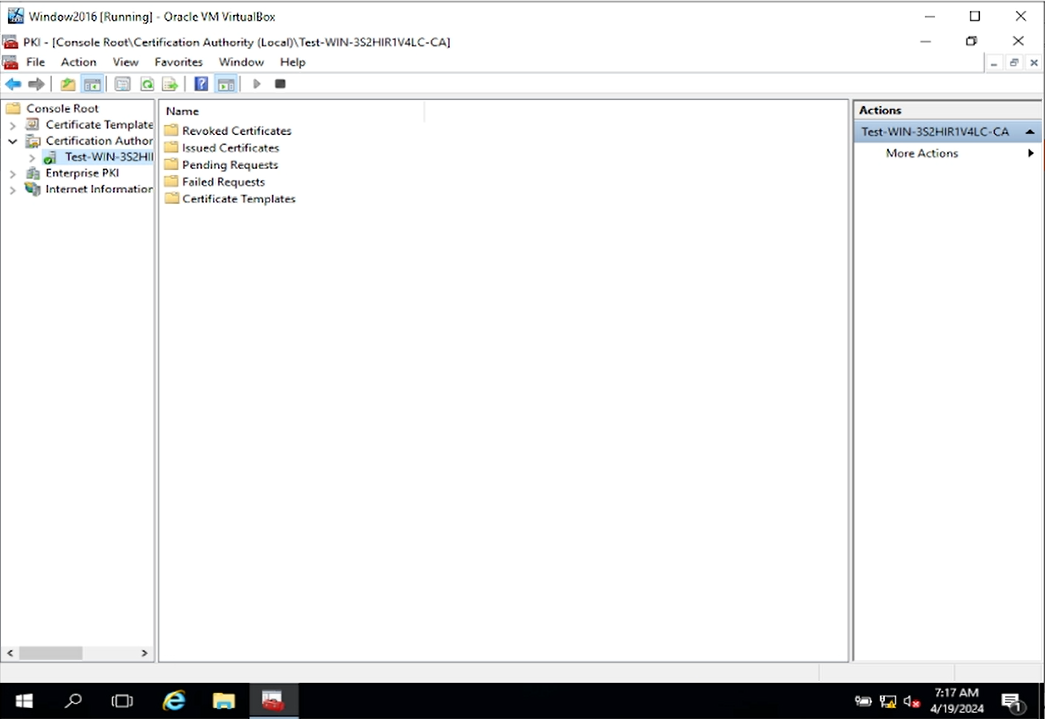
\includegraphics[width=0.9\linewidth]{figure//chapter4//lab4_2/ca_local.png}
    \caption{Thông tin trong Certification Authority (Local)}
    \label{fig:enter-label}
\end{figure}

\noindent {\bf{Bước 4:}} Mở rộng phần \textbf{Certificate Templates} ở trong mục Certification Authority (Local)/ServerName. Mở rộng các file này và tìm hiểu.

\begin{figure}[!htb]
    \centering
    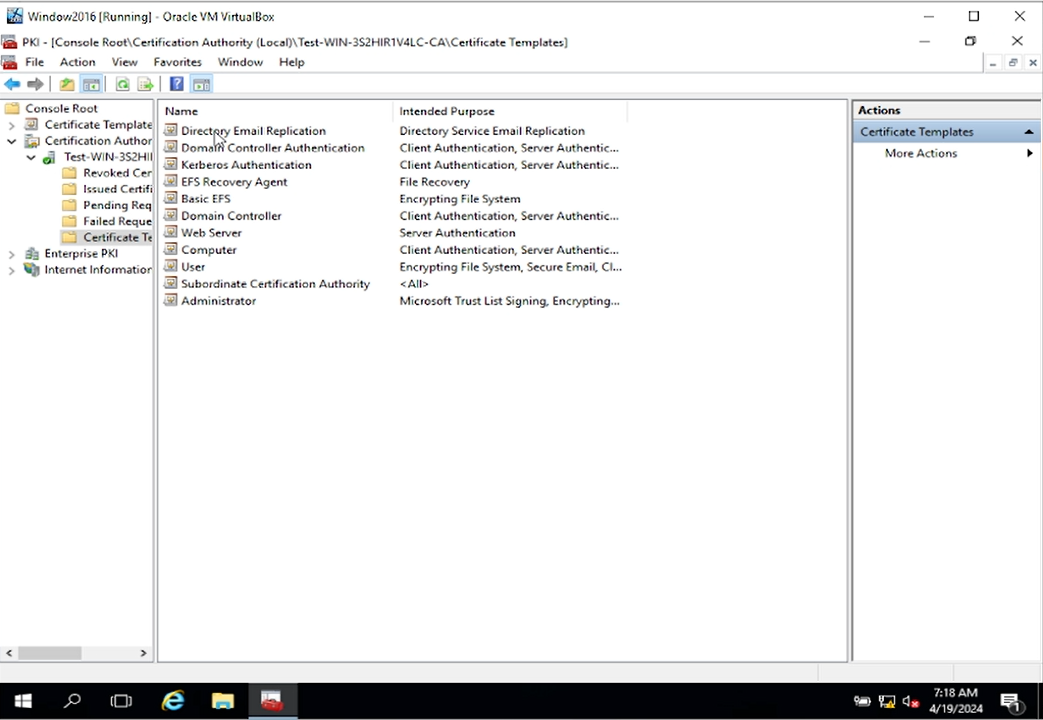
\includegraphics[width=0.9\linewidth]{figure//chapter4//lab4_2/cert_temp.png}
    \caption{Thông tin trong Certificate Templates}
    \label{fig:enter-label}
\end{figure}

\noindent {\bf{Bước 5:}} Vào Start, chọn \textbf{Windows Administrative Tools}, chọn \textbf{Internet Information Services (IIS) Manager}. Ở thanh Connection, chọn ServerName, mở rộng Sites và Default Web Site.

\begin{figure}[!htb]
    \centering
    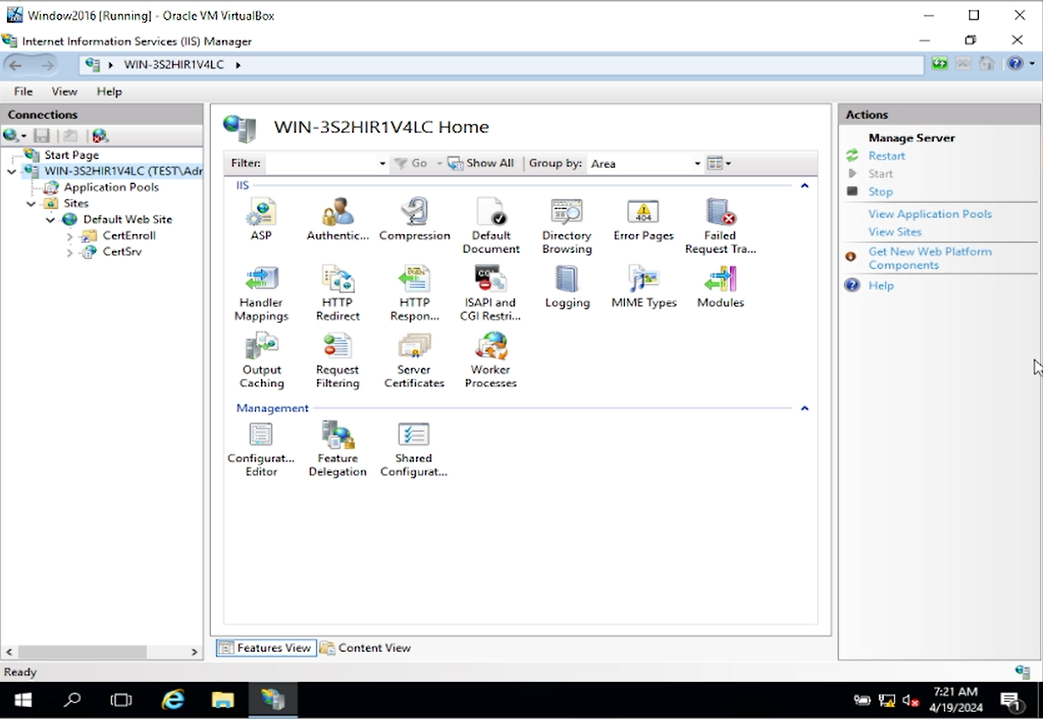
\includegraphics[width=0.9\linewidth]{figure//chapter4//lab4_2/iis_manager.png}
    \caption{Thông tin trong IIS Manager}
    \label{fig:enter-label}
\end{figure}

\noindent {\bf{Bước 6:}} Chọn Authentication. Chắc chắn rằng \textbf{Anonymous Authentication} đã được bật.

\begin{figure}[!htb]
    \centering
    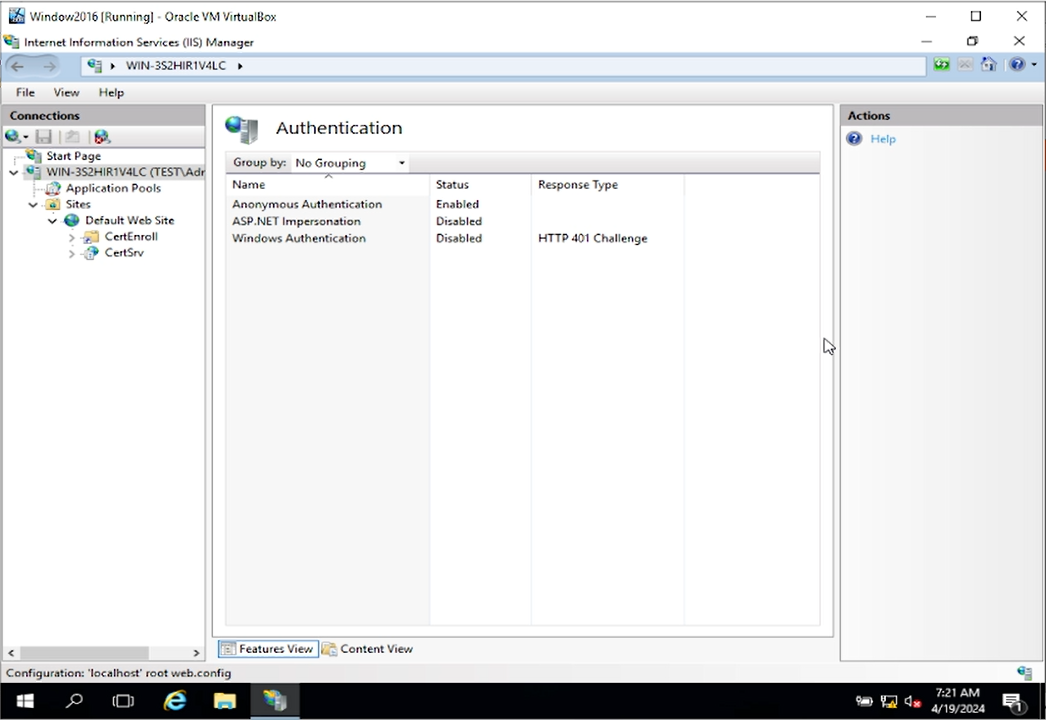
\includegraphics[width=0.8\linewidth]{figure//chapter4//lab4_2/iis_auth.png}
    \caption{Màn hình Authentication trong IIS Manager}
    \label{fig:enter-label}
\end{figure}

\newpage
\noindent {\bf{Bước 7:}} Chọn \textbf{Default Web Site}, chọn \textbf{Authentication}. Kiểm tra \textbf{Anonymous Authentication}. Sau đó quay lại, chọn \textbf{SSL Settings}.

\begin{figure}[!htb]
    \centering
    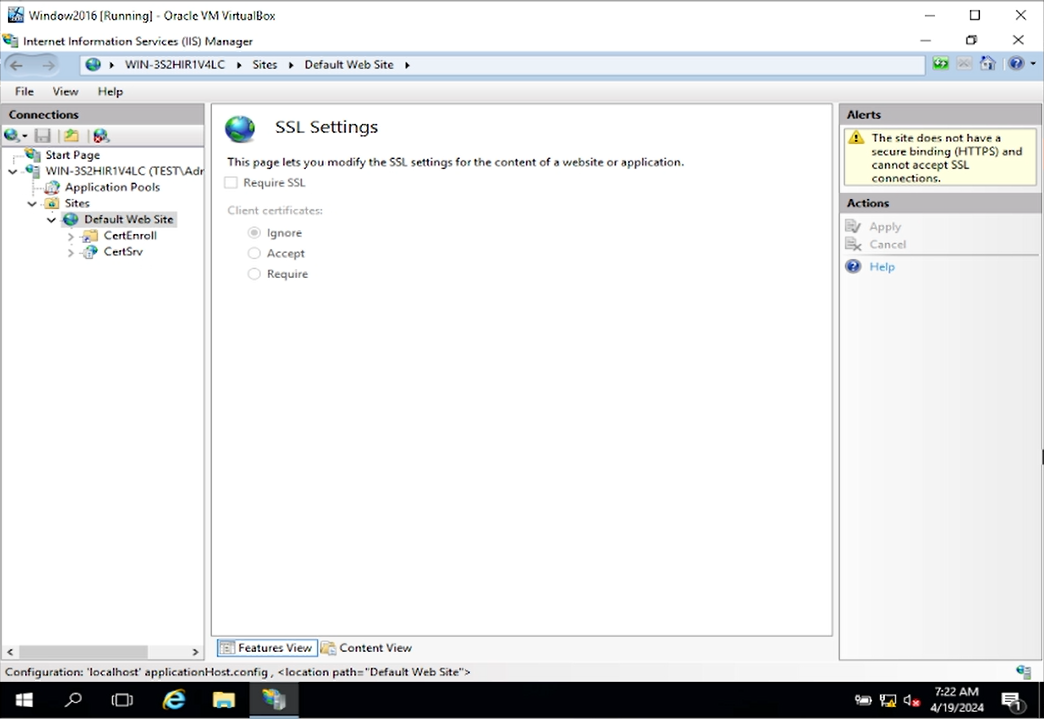
\includegraphics[width=0.8\linewidth]{figure//chapter4//lab4_2/ssl_settings.png}
    \caption{Màn hình SSL Settings}
    \label{fig:enter-label}
\end{figure}

\noindent Tại đây, bạn có thể thấy các mục bị mờ đi. Lý do là bởi đang không có binding HTTPS và web server certificate tới port 443. Để thêm binding, ta chọn vào ServerName, chọn Server Certificates. Trong trường hợp chỉ có 1 certificate, reboot máy ảo. Sau đó, ta có thể nhấn vào các certificate để biết thêm thông tin.

\begin{figure}[!htb]
    \centering
    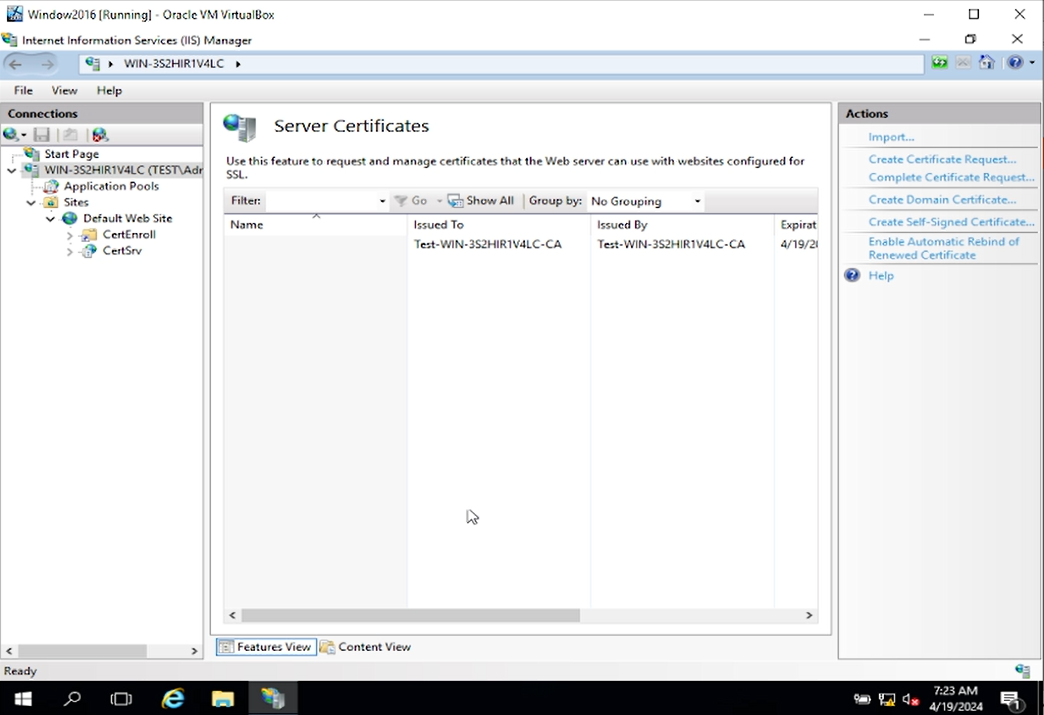
\includegraphics[width=0.8\linewidth]{figure//chapter4//lab4_2/ser_cert.png}
    \caption{Các certificate trong Server Certificates}
    \label{fig:enter-label}
\end{figure}

\newpage

\noindent {\bf{Bước 8:}} Chọn \textbf{Default Web Site}. Chọn \textbf{Bindings} ở thanh \textbf{Actions} ở phía bên phải.

\begin{figure}[!htb]
    \centering
    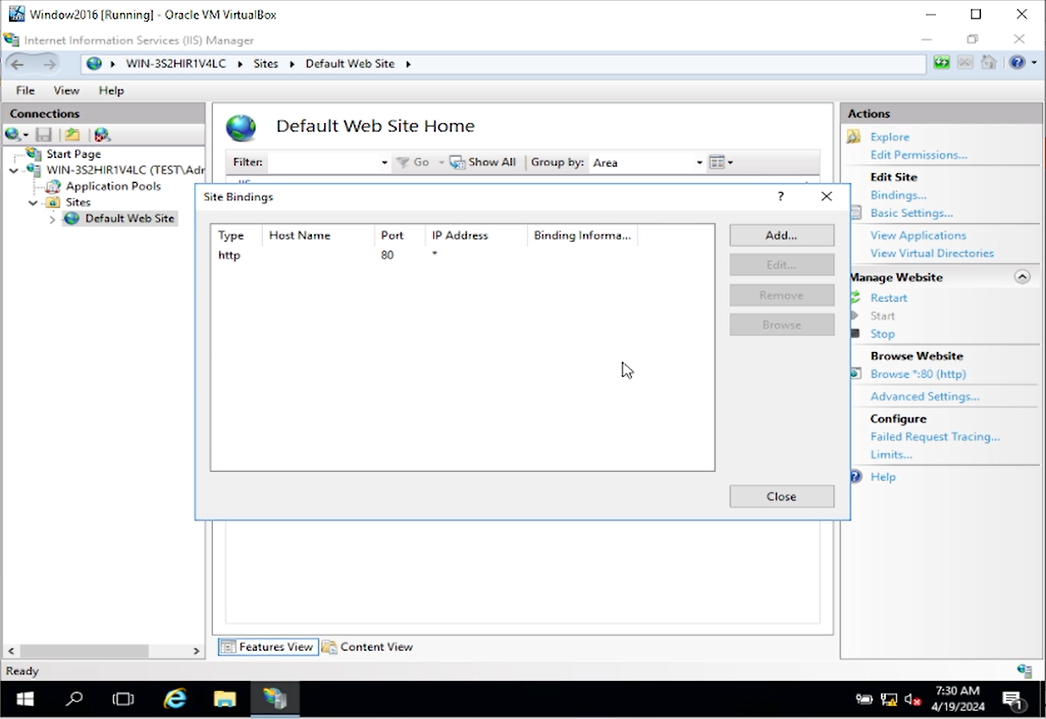
\includegraphics[width=0.9\linewidth]{figure//chapter4//lab4_2/bindings.png}
    \caption{Màn hình Bindings}
    \label{fig:enter-label}
\end{figure}

\noindent {\bf{Bước 9:}} Chọn \textbf{Add}, chọn \textbf{https} ở \textbf{Type} cho port 443. Chọn SSL Certificates tương ứng với ServerName. Click \textbf{OK}.

\begin{figure}[!htb]
    \centering
    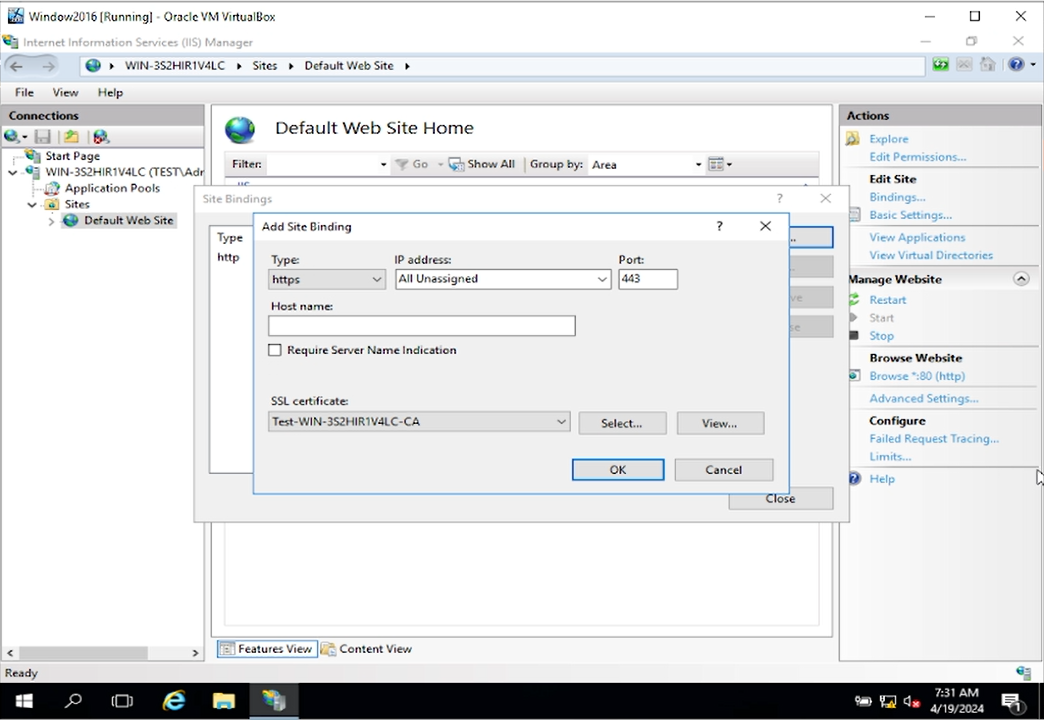
\includegraphics[width=0.9  \linewidth]{figure//chapter4//lab4_2/add_bindings.png}
    \caption{Thêm Binding}
    \label{fig:enter-label}
\end{figure}

\noindent {\bf{Bước 10:}} Quay lại \textbf{SSL Settings} trong \textbf{Default Web Site}. Lúc này các mục không còn mờ nữa. Chọn \textbf{Require SSL} và nhấn \textbf{Apply}.

\begin{figure}[!htb]
    \centering
    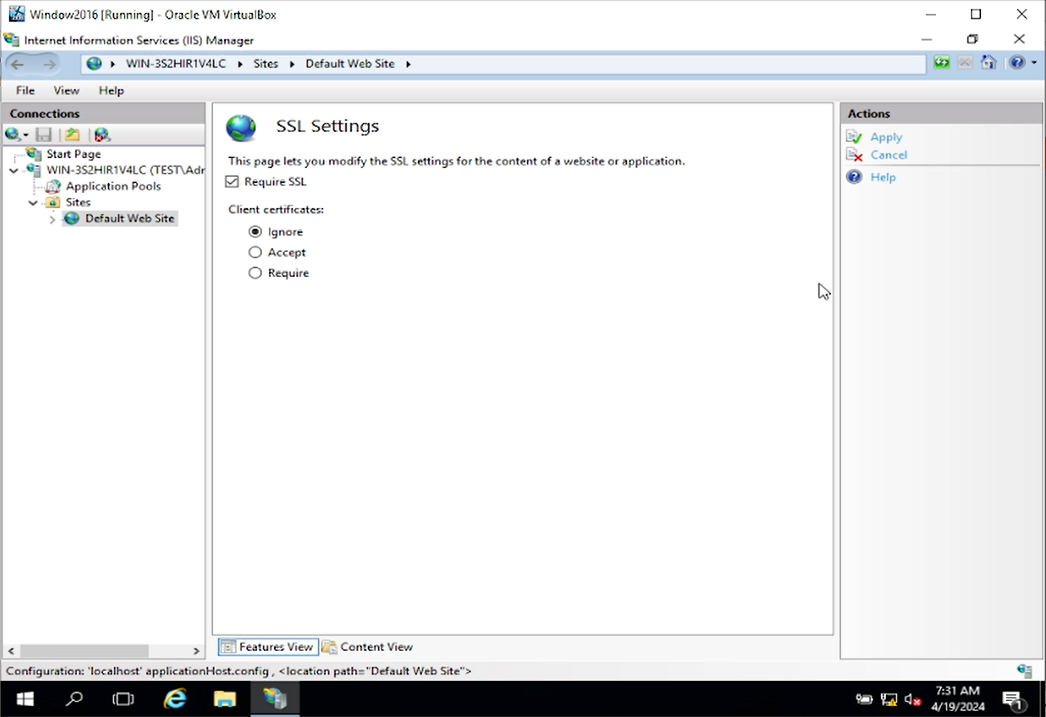
\includegraphics[width=0.9\linewidth]{figure//chapter4//lab4_2/ssl_setting_after_bind.png}
    \caption{Màn hình SSL Settings sau khi thực hiện thêm Binding}
    \label{fig:enter-label}
\end{figure}

\noindent {\bf{Bước 11:}} Vào \textbf{Start}, chọn \textbf{Active Directory Users and Computers}. Sau đó tạo người dùng mới. Đặt tên là Anthony Newman, username là anewman, mật khẩu là Pa\$\$word. Sau đó click vào tài khoản của Anthony Newman và điền email là anewman@teamx.net. 

\begin{figure}[!htb]
    \centering
    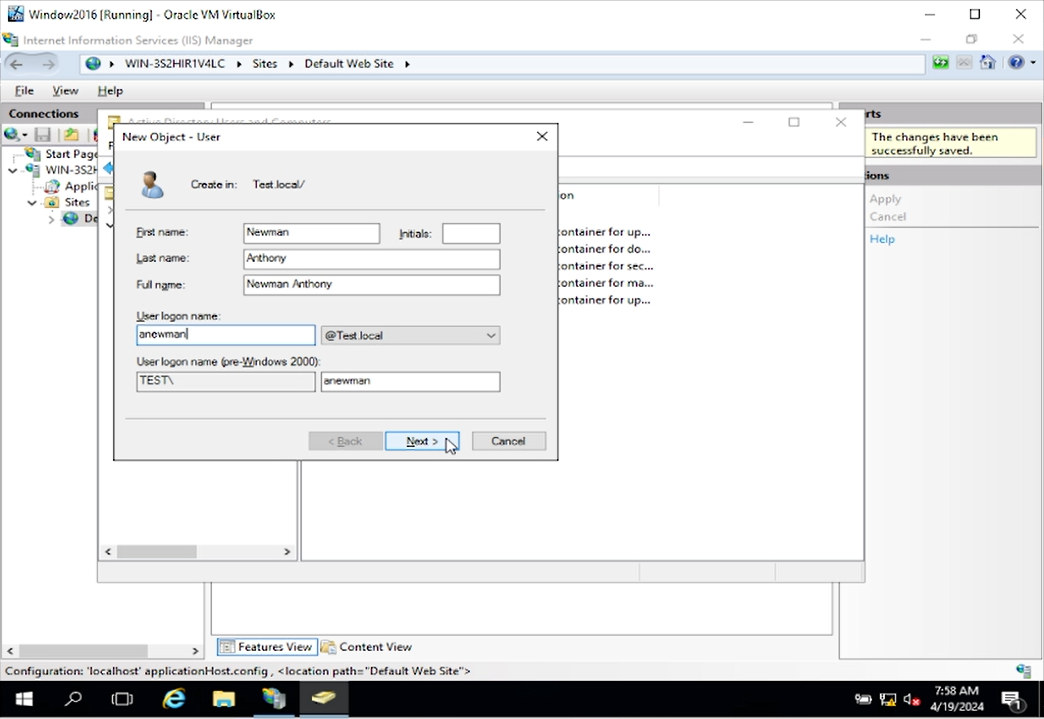
\includegraphics[width=0.8\linewidth]{figure//chapter4//lab4_2/create_account.png}
    \caption{Tạo người dùng mới}
    \label{fig:enter-label}
\end{figure}

\subsection{Review Questions}

\noindent Câu 1: 

D: The client and web server exchanging root certificates.

\noindent Câu 2: 

D: 443.

\noindent Câu 3: 

D: No port had been configured to "listen" for https requests.

\noindent Câu 4: 

C: To have a location for centralized account maintenance.

\noindent Câu 5: True.
\section{GOST Hash Function}
\subsection{Activities}

None

\subsection{Review Questions}

\noindent Câu 1: 

B: $2^{128}$.

\noindent Câu 2: 

D: 256.

\noindent Câu 3: True.

\noindent Câu 4: 

A. Block.

\noindent Câu 5: True.
\newpage
\section{Configuring Certificate Auto-Enrollment}
\subsection{Activities}

\noindent {\bf{Bước 1:}} Khởi động máy ảo Windows được sử dụng trong phần 2.

\noindent {\bf{Bước 2:}} Mở PKI, thên snap-in \textbf{Group Policy Management} theo cách được sử dụng trong phần 2.

\begin{figure}[!htb]
    \centering
    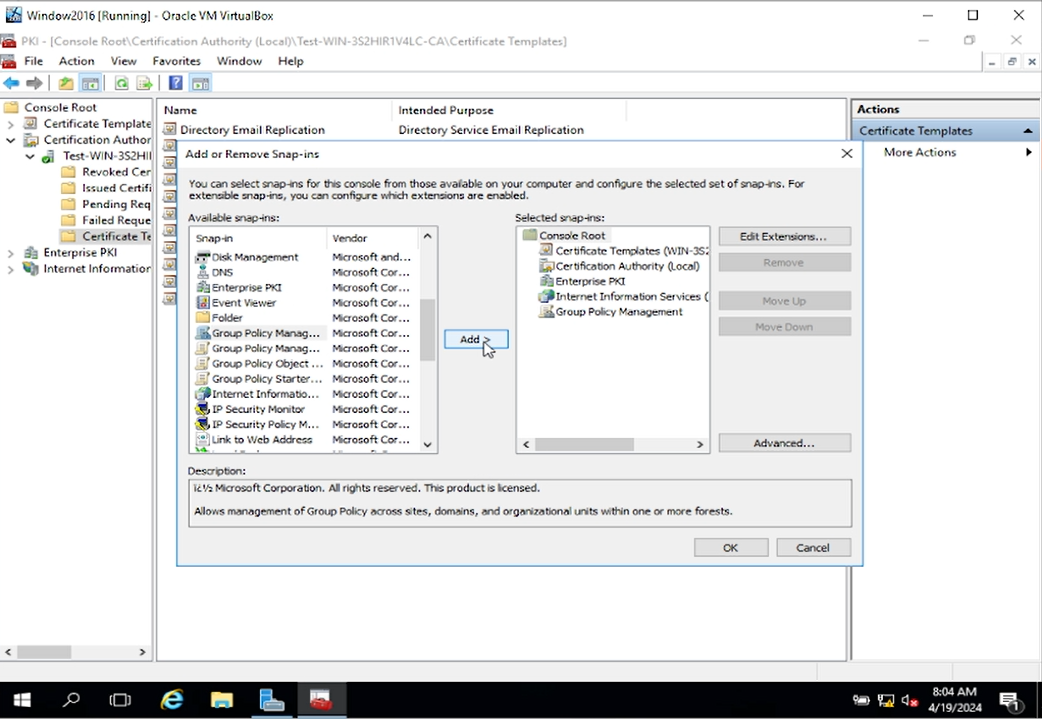
\includegraphics[width=0.7\linewidth]{figure//chapter4//lab4_3/add_group_policy_management.png}
    \caption{Thêm Group Policy Management}
    \label{fig:enter-label}
\end{figure}

\noindent {\bf{Bước 3:}} Ở PKI, mở rộng\textbf{Group Policy Management} > \textbf{Forest.local} > \textbf{Domains} > \textbf{Test.local}. Chuột phải \textbf{Default Domain Policy}, chọn \textbf{Edit}. 

\begin{figure}[!htb]
    \centering
    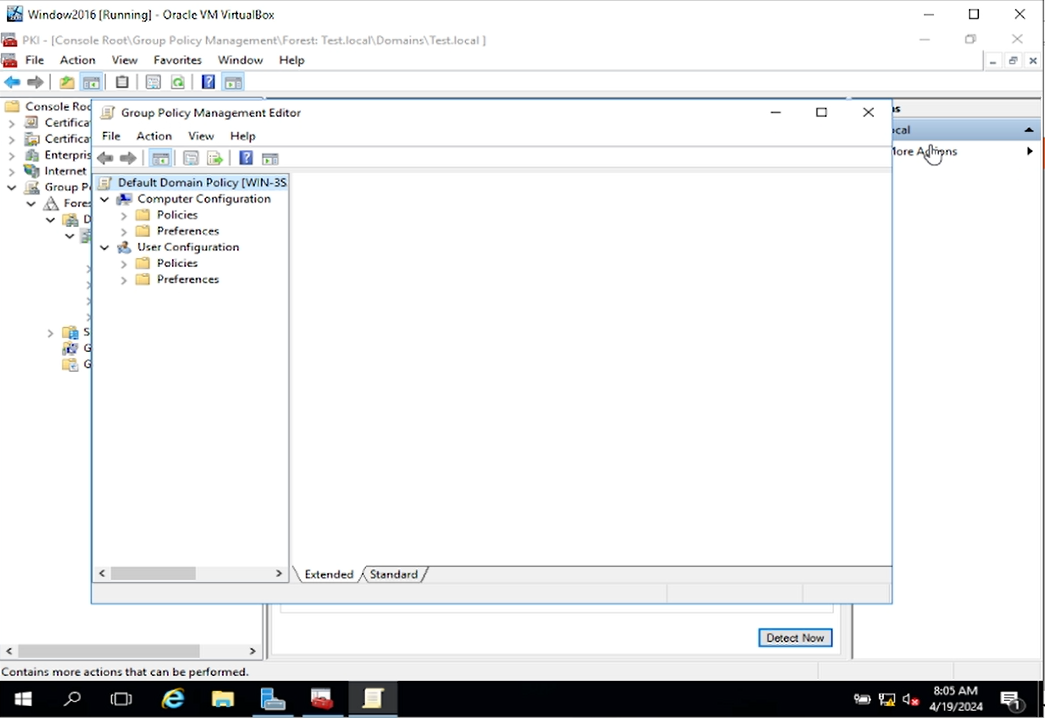
\includegraphics[width=0.8\linewidth]{figure//chapter4//lab4_3/gpm_editor.png}
    \caption{Màn hình Group Policy Management Editor}
    \label{fig:enter-label}
\end{figure}

Tiếp tục mở rộng theo thứ tự \textbf{User Configuration } > \textbf{Policies} > \textbf{Windows Settings} > \textbf{Security Settings} và chọn \textbf{Public Key Policies}.

\begin{figure}[!htb]
    \centering
    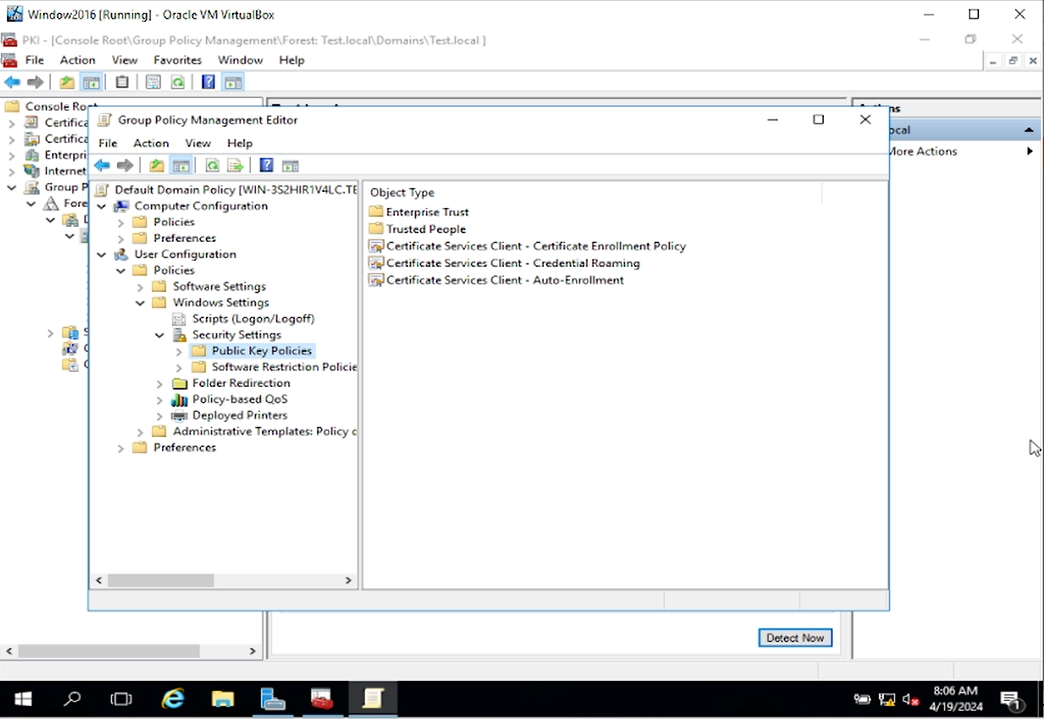
\includegraphics[width=0.8\linewidth]{figure//chapter4//lab4_3/public_key_policies.png}
    \caption{Public Key Policies}
    \label{fig:enter-label}
\end{figure}

Ở thanh bên phải, chuột phải vào \textbf{Certificate Services Client -  AutoEnrollment} và chọn \textbf{Properties}. Đặt \textbf{Configuration Model} thành \textbf{Enable} và chọn \textbf{Renew expired certificates, update pending certificates, and remove revoked certificates} và \textbf{Update certificates that use certificate templates}.

\begin{figure}[!htb]
    \centering
    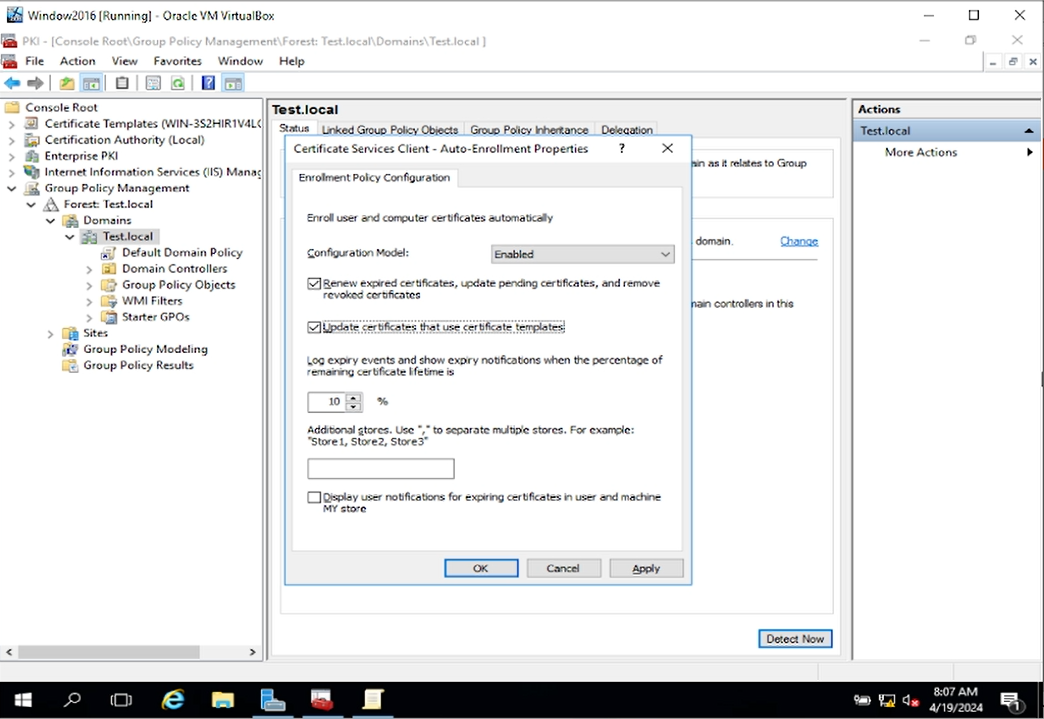
\includegraphics[width=0.8\linewidth]{figure//chapter4//lab4_3/cert_service_client_autoenrollment.png}
    \caption{Cấu hình Certificate Service Client Auto-Enrollment}
    \label{fig:enter-label}
\end{figure}

\newpage

\noindent {\bf{Bước 4:}} Ở PKI, mở rộng \textbf{Certification Authority (Local)} > ServerName, chọn \textbf{Certificate Templates}.

\begin{figure}[!htb]
    \centering
    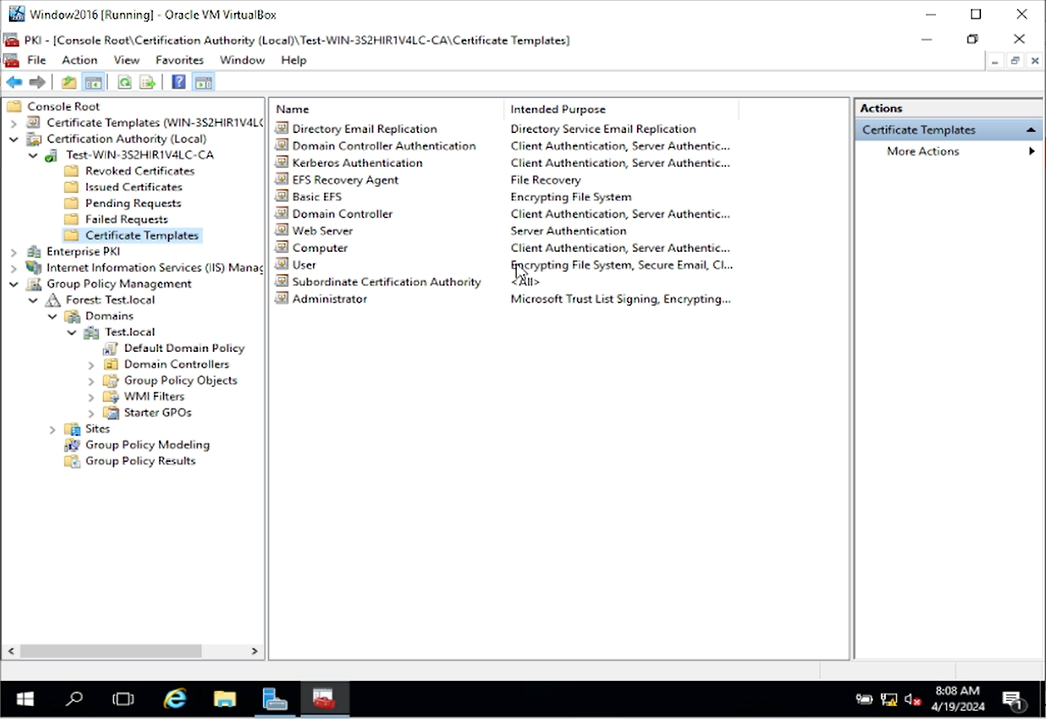
\includegraphics[width=0.9\linewidth]{figure//chapter4//lab4_3/cert_temp_in_auth.png}
    \caption{Màn hình Certificate Templates trong phần Certification Authority (Local)}
    \label{fig:enter-label}
\end{figure}

\noindent {\bf{Bước 5:}} Chọn \textbf{Certificate Templates} ở bên ngoài, chuột phải vào User và chọn \textbf{Duplicate Template}.

\begin{figure}[!htb]
    \centering
    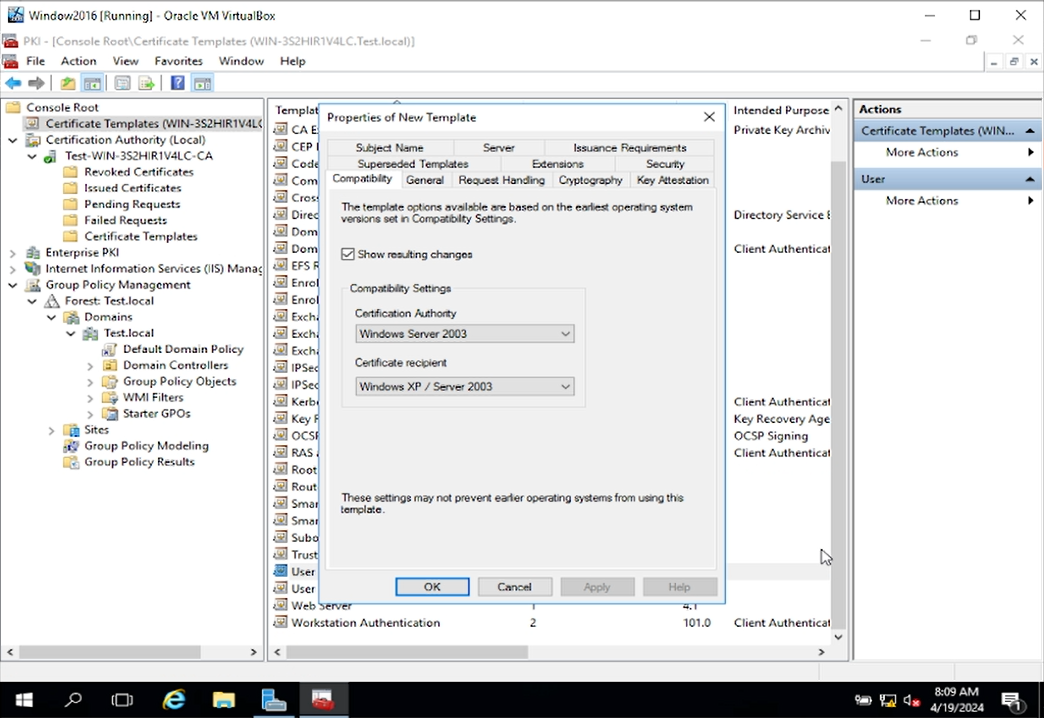
\includegraphics[width=0.9\linewidth]{figure//chapter4//lab4_3/duplicate_template.png}
    \caption{Màn hình Duplicate Template}
    \label{fig:enter-label}
\end{figure}

Ở \textbf{General}, chuyển \textbf{Template display name} thành \textbf{ServerName}, \textbf{Validity period number} thành 2 năm, và \textbf{Renewal period number} thành 12 tháng.

\begin{figure}[!htb]
    \centering
    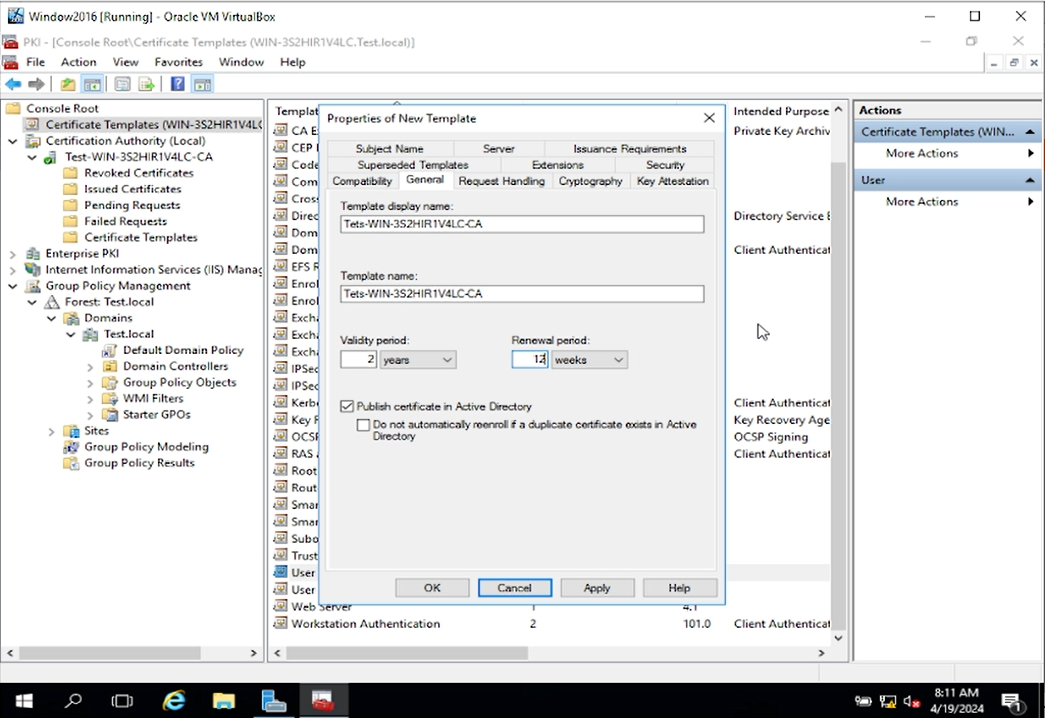
\includegraphics[width=0.9\linewidth]{figure//chapter4//lab4_3/general_tab.png}
    \caption{General Tab}
    \label{fig:enter-label}
\end{figure}

Ở \textbf{Request Handling}, chọn \textbf{Prompt the user during enrollment}.

\begin{figure}[!htb]
    \centering
    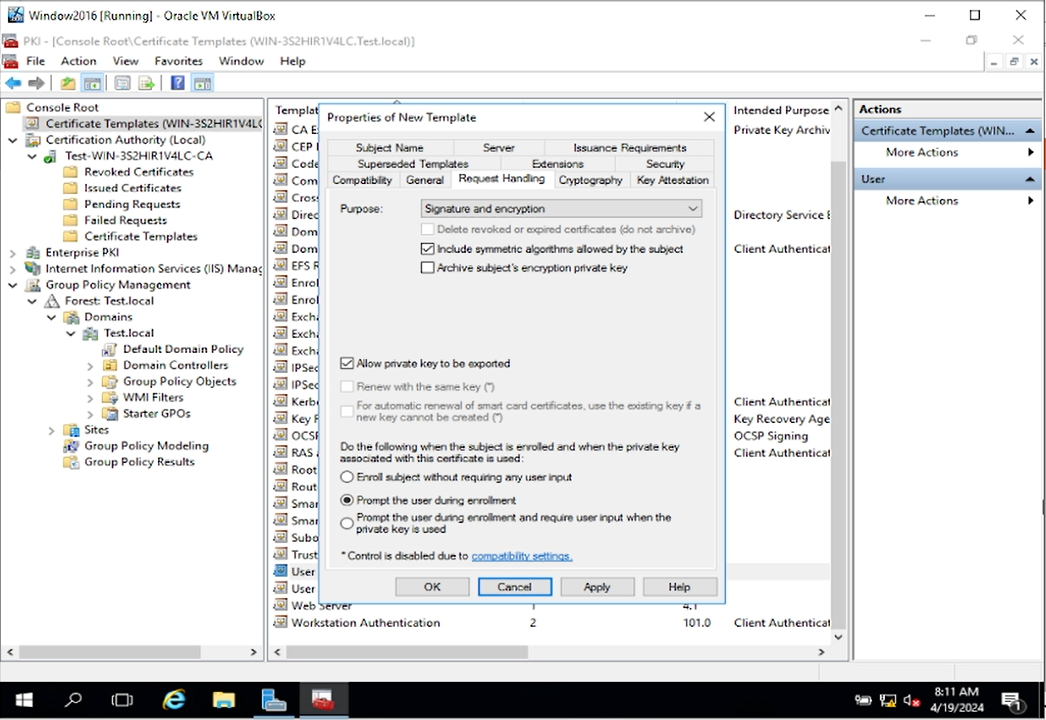
\includegraphics[width=0.9\linewidth]{figure//chapter4//lab4_3/request_handling.png}
    \caption{Request Handling Tab}
    \label{fig:enter-label}
\end{figure}

\noindent {\bf{Bước 6:}} Ở \textbf{Security}, chọn \textbf{Add}. Chuyển \textbf{Enter the object names to select box} thành \textbf{Anthony Newman} (Tài khoản đã được lập trước đó). Ở \textbf{Group or user names}, chọn Anthony Newman. Và ở \textbf{Permissions for Anthony Newman}, chọn \textbf{Allow} cho \textbf{Enroll} và \textbf{Autoenroll}.

\begin{figure}[!htb]
    \centering
    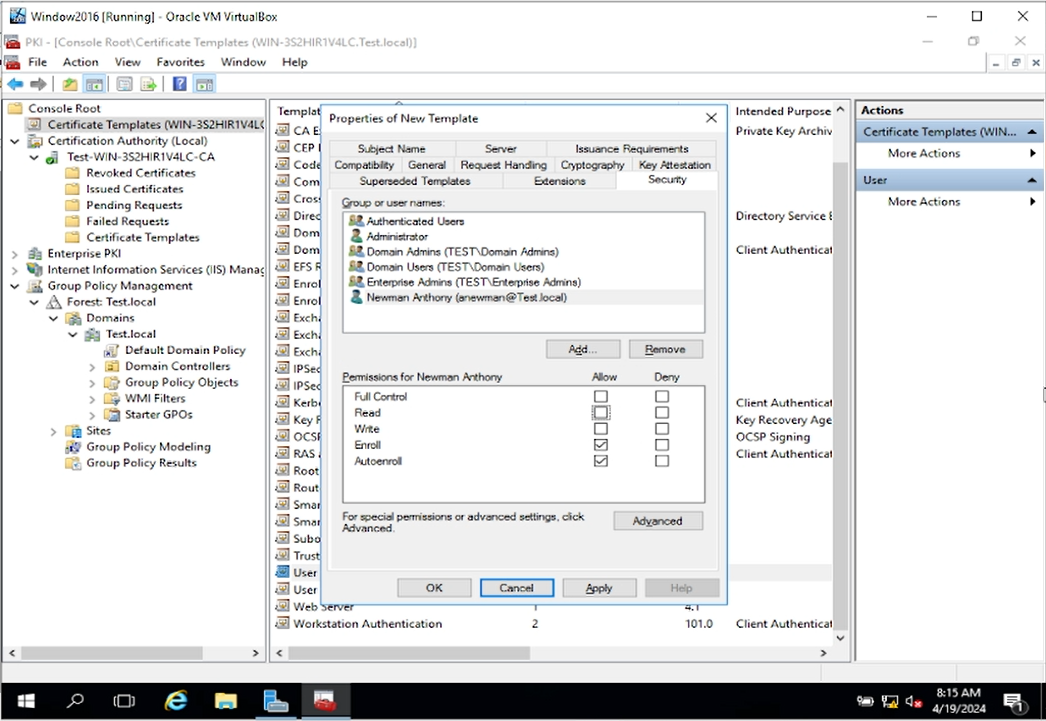
\includegraphics[width=0.7\linewidth]{figure//chapter4//lab4_3/security_tab.png}
    \caption{Security Tab}
    \label{fig:enter-label}
\end{figure}

\noindent {\bf{Bước 7:}} Quay lại \textbf{Certificate Templates} ở trong \textbf{Certification Authority (Local)}. Nhấn chuột phải và chọn \textbf{New}, chọn \textbf{Certificate Template to Issue}. Ở \textbf{Enable Certificate Templates}, chọn \textbf{ServerName}. Certificate mới sẽ xuất hiện ở \textbf{Certificate Templates}.

\begin{figure}[!htb]
    \centering
    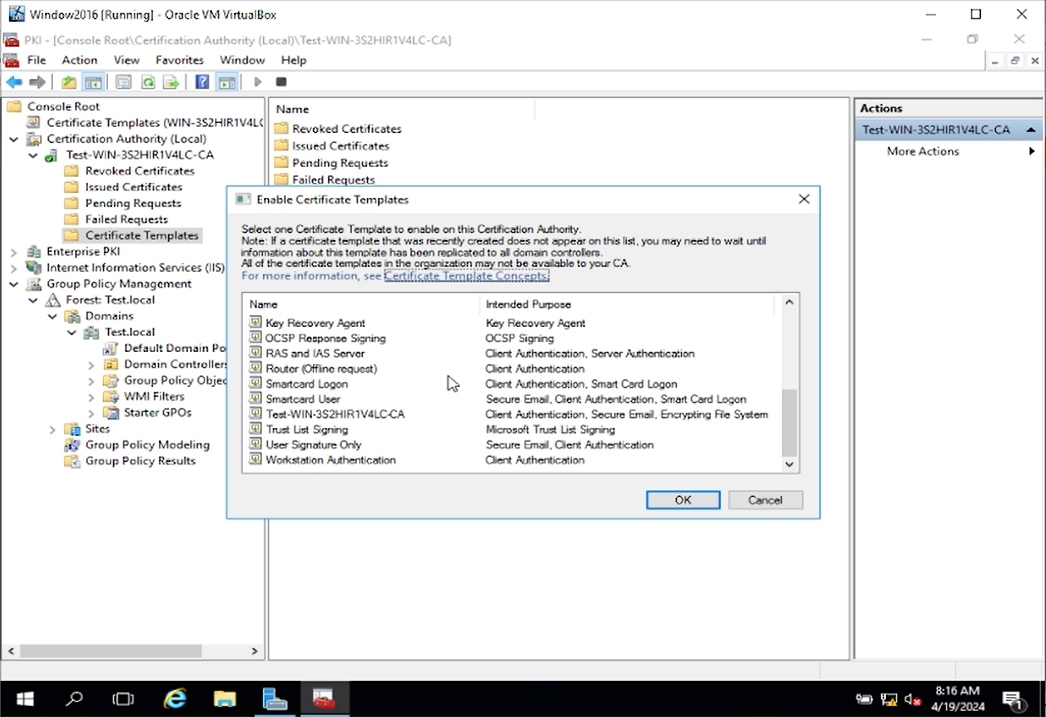
\includegraphics[width=0.7\linewidth]{figure//chapter4//lab4_3/enable_certificate.png}
    \caption{Màn hình Enable Certificate Templates}
    \label{fig:enter-label}
\end{figure}

Cuối cùng, có thể click vào \textbf{ServerName} để biết thêm chi tiết về Certificate này.

\subsection{Review Questions}

\noindent Câu 1: 

A: Users should export their public keys and store them in a safe place.

\noindent Câu 2: 

ii: Choose a certificate template that allow users to digitally sign emails.

B: you did not assign the global security group the View permission to the certificate template.

\noindent Câu 3: 

B: Once a User certificate is issued to a user, the best practice is to revoke the user's EFS certiciate.

\noindent Câu 4: True.

\noindent Câu 5:

B: Install Anthony's certificate.
\newpage

\section{Getting started with Kali Linux}
\subsection{Activity}

\noindent {\bf{Bước 1:}} Truy cập vào đường dẫn \href{https://old.kali.org/kali-images/kali-2016.2/}{Link} và chọn phiên bản Kali Linux 2016 phù hợp rồi tải về.

\begin{figure}[!htb]
    \centering
    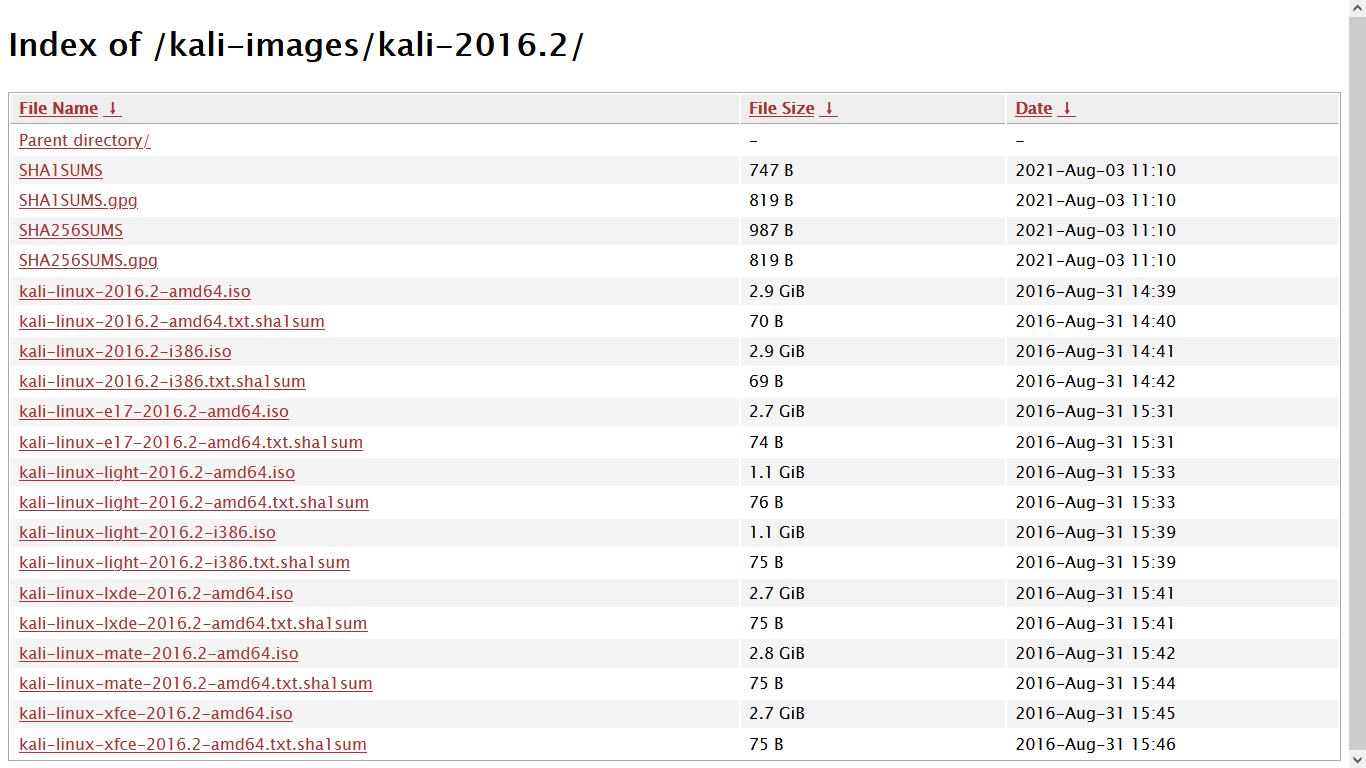
\includegraphics[width=0.9\linewidth]{figure//chapter5//lab5_1/download_kali_linux.png}
    \caption{Tải Kali Linux 2016}
    \label{fig:enter-label}
\end{figure}

\noindent {\bf{Bước 2:}} Cấu hình máy ảo và khởi động. Chọn máy ảo Linux, phiên bản Linux 2.6/3.x/4.x/5.x. Cấp 25GB bộ nhớ, 2 cpu. Tạo máy ảo và khởi động.

\begin{figure}[!htb]
    \centering
    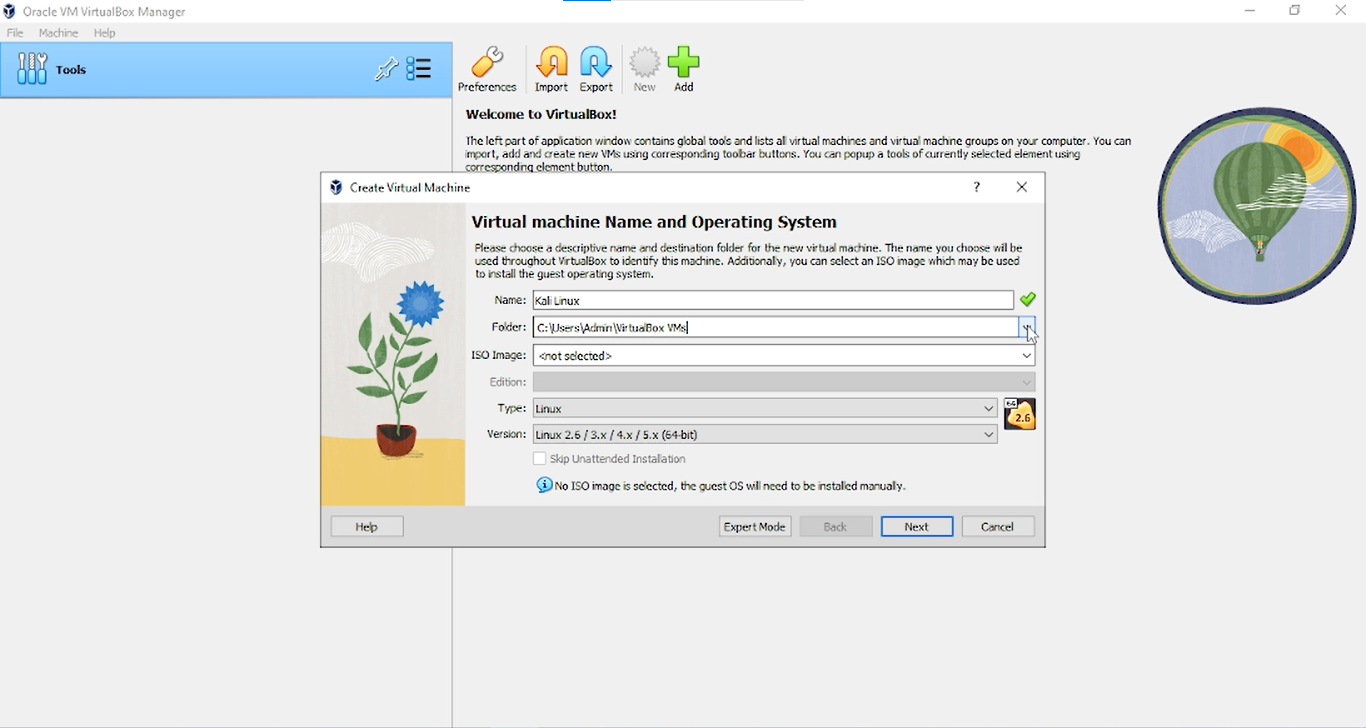
\includegraphics[width=0.9\linewidth]{figure//chapter5//lab5_1/create_vm.png}
    \caption{Tạo máy ảo}
    \label{fig:enter-label}
\end{figure}

\newpage

\noindent {\bf{Bước 3:}} Sau khi khởi động xong, chọn \textbf{Graphical Install}.

\begin{figure}[!htb]
    \centering
    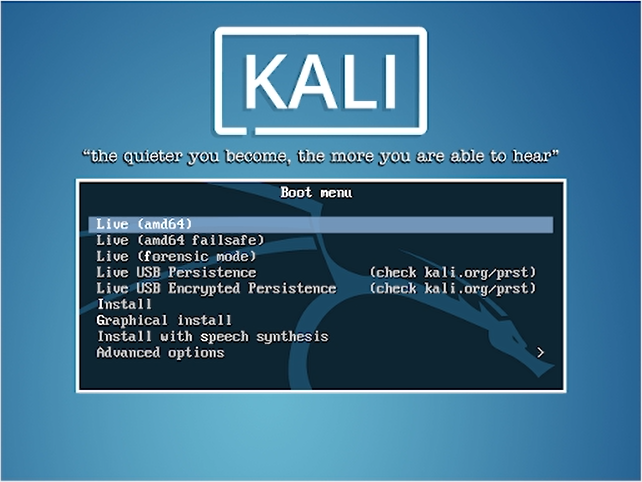
\includegraphics[width=0.85\linewidth]{figure//chapter5//lab5_1/graphical_install.png}
    \caption{Boot options}
    \label{fig:enter-label}
\end{figure}

\noindent {\bf{Bước 4:}} Tiếp tục với các cài đặt mặc định. Tại \textbf{Configure the network}, nhập \textbf{Test.com} và \textbf{Continue}. Sau đó nhập mật khẩu là \textbf{admin}.

\begin{figure}[!htb]
    \centering
    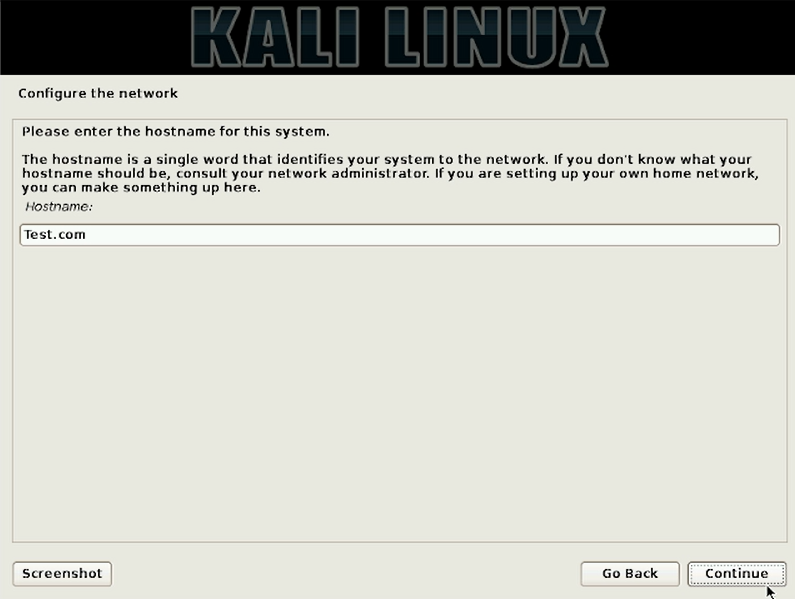
\includegraphics[width=0.85\linewidth]{figure//chapter5//lab5_1/configure_network.png}
    \caption{Cấu hình mạng}
    \label{fig:enter-label}
\end{figure}

\noindent {\bf{Bước 5:}} Tại \textbf{Partition disks}, chọn \textbf{Yes}.

\begin{figure}[!htb]
    \centering
    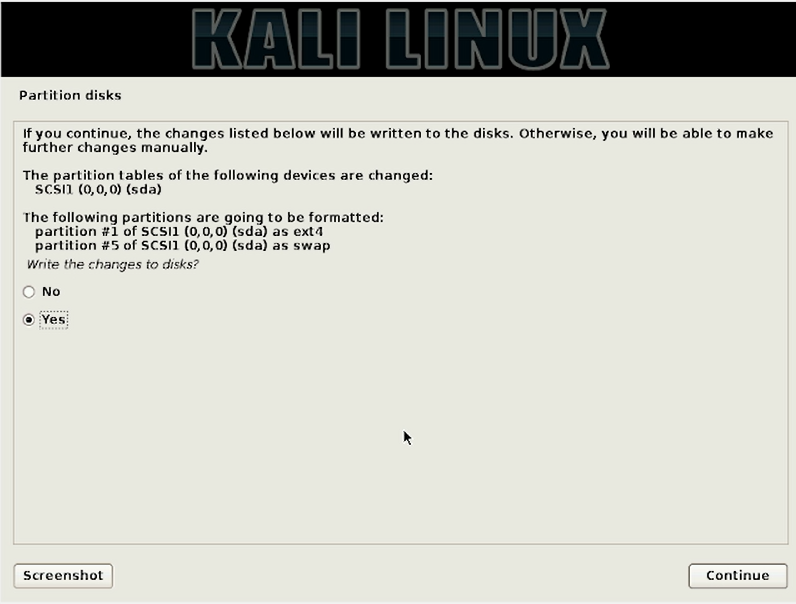
\includegraphics[width=0.85\linewidth]{figure//chapter5//lab5_1/partition_disk.png}
    \caption{Partition Disks Configuration}
    \label{fig:enter-label}
\end{figure}

\noindent {\bf{Bước 6:}} Tại \textbf{Configre the package manager}, chọn \textbf{No}.

\begin{figure}[!htb]
    \centering
    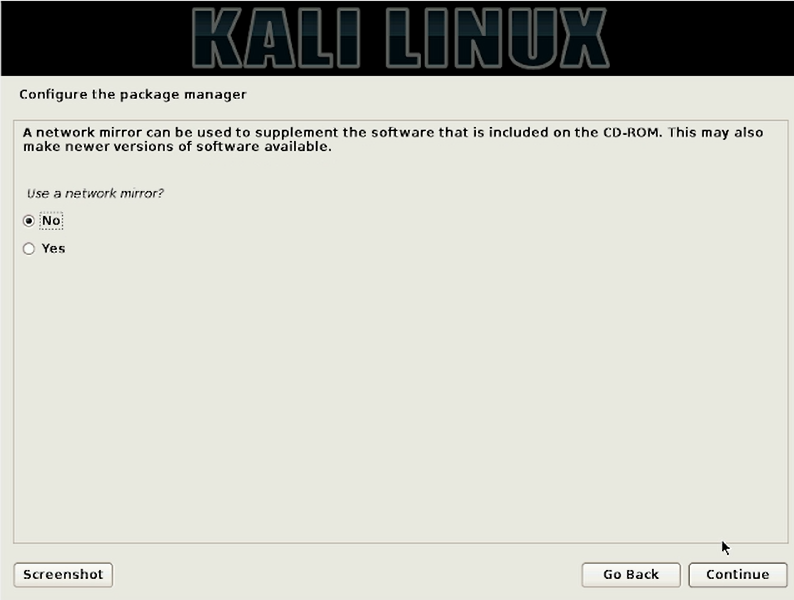
\includegraphics[width=0.85\linewidth]{figure//chapter5//lab5_1/package_manager.png}
    \caption{Package Manager Configuration}
    \label{fig:enter-label}
\end{figure}

\newpage

\noindent {\bf{Bước 7:}} Tại \textbf{GRUB boot loader}, chọn \textbf{Yes}. Sau đó chọn các cài đặt mặc định và \textbf{Install}. Cuối cùng khởi động lại máy.

\begin{figure}[!htb]
    \centering
    \includegraphics[width=0.85\linewidth]{figure//chapter5//lab5_1/GRUB.png}
    \caption{GRUB Boot Loader}
    \label{fig:enter-label}
\end{figure}

\noindent {\bf{Bước 8:}} Nhập \textbf{root} và \textbf{admin} để đăng nhập vào hệ thống.

\begin{figure}[!htb]
    \centering
    \includegraphics[width=0.85\linewidth]{figure//chapter5//lab5_1/login.png}
    \caption{Login to Linux}
    \label{fig:enter-label}
\end{figure}

\noindent {\bf{Bước 9:}} Mở \textbf{Terminal}.

\begin{figure}[!htb]
    \centering
    \includegraphics[width=0.85\linewidth]{figure//chapter5//lab5_1/terminal.png}
    \caption{Mở Terminal}
    \label{fig:enter-label}
\end{figure}

\noindent {\bf{Bước 10:}} Nhập \textbf{ifconfig}. Nếu inet addr bằng 127.0.0.1, thì tức là bạn phải cấu hình địa chỉ IP thủ công.

\begin{figure}[!htb]
    \centering
    \includegraphics[width=0.85\linewidth]{figure//chapter5//lab5_1/manual_configure.png}
    \caption{Kết quả khi thực hiện ifconfig}
    \label{fig:enter-label}
\end{figure}

\newpage

\noindent {\bf{Bước 11:}} Nhập \textbf{/etc/init.d/networking start} để bắt đầu dịch vụ mạng.

\begin{figure}[!htb]
    \centering
    \includegraphics[width=0.85\linewidth]{figure//chapter5//lab5_1/networking_service.png}
    \caption{Khởi động dịch vụ mạng}
    \label{fig:enter-label}
\end{figure}

\noindent {\bf{Bước 12:}} Ở VirtualBox, chọn \textbf{Machine/Settings/Network}. Chắc VM đã nhận ra được Adapter của máy bạn.

\begin{figure}[!htb]
    \centering
    \includegraphics[width=0.85\linewidth]{figure//chapter5//lab5_1/vm_network.png}
    \caption{Network trong VirtualBox}
    \label{fig:enter-label}
\end{figure}

\newpage

\noindent {\bf{Bước 13:}} Ping \textbf{www.yahoo.com} để kiểm tra.

\begin{figure}[!htb]
    \centering
    \includegraphics[width=0.85\linewidth]{figure//chapter5//lab5_1/ping_yahoo.png}
    \caption{Ping Yahoo}
    \label{fig:enter-label}
\end{figure}

\noindent {\bf{Bước 14:}} Chạy ứng dụng \textbf{ZenMap} trong \textbf{Application/Information Gathering}.

\begin{figure}[!htb]
    \centering
    \includegraphics[width=0.85\linewidth]{figure//chapter5//lab5_1/zenmap.png}
    \caption{Chạy ứng dụng Zenmap}
    \label{fig:enter-label}
\end{figure}

\noindent {\bf{Bước 15:}} Ở phần \textbf{Target}, nhập \textbf{uet.vnu.edu.vn}. Sau đó chọn \textbf{Scan}.

\begin{figure}[!htb]
    \centering
    \includegraphics[width=0.85\linewidth]{figure//chapter5//lab5_1/scan-site.png}
    \caption{Scan uet.vnu.edu.vn}
    \label{fig:enter-label}
\end{figure}

\noindent {\bf{Bước 16:}} Chọn \textbf{Topology}. Tại đây, ta sẽ thấy các lần nhảy để tới được địa chỉ web đó.

\begin{figure}[!htb]
    \centering
    \includegraphics[width=0.85\linewidth]{figure//chapter5//lab5_1/topology.png}
    \caption{Màn hình Topology}
    \label{fig:enter-label}
\end{figure}

\newpage

\noindent {\bf{Bước 17:}} Mở \textbf{Nmap Output} và kiểm tra thêm các output.

\begin{figure}[!htb]
    \centering
    \includegraphics[width=0.85\linewidth]{figure//chapter5//lab5_1/nmap-output.png}
    \caption{Nmap Output}
    \label{fig:enter-label}
\end{figure}

\subsection{Review Questions}

\noindent Câu 1: 

B: BackTrack.

\noindent Câu 2: True.

\noindent Câu 3: 

D: GVim.

\noindent Câu 4:

C: 64.

\noindent Câu 5:

D: ls /etc.

\newpage

\section{IP Spoofing with Hping3}

\subsection{Activity}

\noindent {\bf{Bước 1:}} Vào \textbf{VirtualBox}. Chọn Windows Server được tạo từ phần 1. Sau đó cài đặt Network thành \textbf{NAT Network}.

\begin{figure}[!htb]
    \centering
    \includegraphics[width=0.7\linewidth]{figure//chapter5//lab5_1/nat_network.png}
    \caption{Cài đặt NAT Network}
    \label{fig:enter-label}
\end{figure}

\noindent Thực hiện tương tự với Kali Linux VM được tạo từ phần 1.

\noindent {\bf{Bước 2:}} Khởi động Windows Server, chọn \textbf{Start} và chọn \textbf{Control Panel}. Chọn \textbf{Ethernet} > \textbf{Properties}. 

\begin{figure}[!htb]
    \centering
    \includegraphics[width=0.7\linewidth]{figure//chapter5//lab5_2/ethernet_properties.png}
    \caption{Ethernet Properties}
    \label{fig:enter-label}
\end{figure}

\newpage

\noindent {\bf{Bước 3}} Chọn \textbf{Internet Protocol Version 4} > Properties. 

\begin{figure}[!htb]
    \centering
    \includegraphics[width=0.85\linewidth]{figure//chapter5//lab5_2/ipv4_properties.png}
    \caption{IPv4 Properties}
    \label{fig:enter-label}
\end{figure}

\noindent {\bf{Bước 4}} Điền IP 192.168.0.1 và subnet mask 255.255.255.0.

\begin{figure}[!htb]
    \centering
    \includegraphics[width=0.85\linewidth]{figure//chapter5//lab5_2/configure_ip.png}
    \caption{Cấu hình IPv4}
    \label{fig:enter-label}
\end{figure}

\newpage

\noindent {\bf{Bước 5}} Tạo một Windows 10 VM khác giống hệt với Windows Server. Sau đó, cấu hình mạng tương tự với các bước trên, chỉ thay bằng địa chỉ IP 192.168.0.2.

\begin{figure}[!htb]
    \centering
    \includegraphics[width=0.85\linewidth]{figure//chapter5//lab5_2/windows10_network.png}
    \caption{Cấu hình mạng Windows 10}
    \label{fig:enter-label}
\end{figure}

\noindent {\bf{Bước 6}} Ở Kali Linux VM, chọn \textbf{Show application} và chọn \textbf{Settings}.

\begin{figure}[!htb]
    \centering
    \includegraphics[width=0.85\linewidth]{figure//chapter5//lab5_2/setting-linux.png}
    \caption{Màn hình Settings của Kali Linux VM}
    \label{fig:enter-label}
\end{figure}

\noindent {\bf{Bước 7}} Chọn Network để cấu hình mạng. Tại \textbf{TPv4}, đặt IP là 192.168.0.3 và subnet mask là 255.255.255.0.

\begin{figure}[!htb]
    \centering
    \includegraphics[width=0.85\linewidth]{figure//chapter5//lab5_2/network-linux.png}
    \caption{Cấu hình mạng trên Kali Linux}
    \label{fig:enter-label}
\end{figure}

\noindent {\bf{Bước 8}} Mở \textbf{Terminal} và nhập \textbf{hping3 --help} để biết thêm thông tin của lệnh này.

\begin{figure}[!htb]
    \centering
    \includegraphics[width=0.8\linewidth]{figure//chapter5//lab5_2/hping3_info.png}
    \caption{Thông tin lệnh hping3}
    \label{fig:enter-label}
\end{figure}

\noindent {\bf{Bước 9}} Nhập \textbf{wireshark} để mở ứng dụng WireShark. Bạn có thể gặp một cảnh báo thì hãy chọn \textbf{OK}.

\begin{figure}[!htb]
    \centering
    \includegraphics[width=0.8\linewidth]{figure//chapter5//lab5_2/wireshark.png}
    \caption{Màn hình và cảnh báo từ WireShark}
    \label{fig:enter-label}
\end{figure}

\noindent {\bf{Bước 10}} Ở \textbf{Terminal}, nhập \textbf{hping3 -s 192.168.0.1} để ping tới Windows Server VM.

\begin{figure}[!htb]
    \centering
    \includegraphics[width=0.8\linewidth]{figure//chapter5//lab5_2/ping_to_windows_server.png}
    \caption{Ping tới máy ảo Windows Server}
    \label{fig:enter-label}
\end{figure}

\newpage

\noindent {\bf{Bước 11}} Quay lại WireShark, chọn \textbf{etho} và nhấn \textbf{Click/Start}. Đợi 10s rồi \textbf{Stop}. Bạn có thể thấy các thông báo khi có packet gửi tới cho Windows Server VM.

\begin{figure}[!htb]
    \centering
    \includegraphics[width=0.8\linewidth]{figure//chapter5//lab5_2/capture_wireshark.png}
    \caption{Màn hình Wireshark khi Capture}
    \label{fig:enter-label}
\end{figure}

\noindent {\bf{Bước 12}} Tiếp theo, bạn sẽ tiến hành gửi các packet tới cho Windows Server từ Kali Linux, nhưng do đang giả mạo IP nên hệ thống sẽ hiện nguồn từ Windows 10 VM thay vì Kali Linux. Chạy \textbf{hping3 -S 192.168.0.2 -a 192.168.0.1}

\begin{figure}[!htb]
    \centering
    \includegraphics[width=0.8\linewidth]{figure//chapter5//lab5_2/spoof.png}
    \caption{Kết quả khi thay đổi địa chỉ IP}
    \label{fig:enter-label}
\end{figure}

\subsection{Review Questions}

\noindent Câu 1: Because it is absent from back table.

\noindent Câu 2: UDP.

\noindent Câu 3: 

A: Clicking the frame, expanding the Transmission Control Protocol node in the middle frame, and seeing that the Flags item lists (RST).

\noindent Câu 4:

A: -f.

\noindent Câu 5:

C: -K.


\newpage

\section{ARP Poisoning}
\subsection{Activity}

\noindent {\bf{Bước 1:}} Khởi động Kali Linux VM từ phần 2. Vào \textbf{Terminal}, nhập lệnh \textbf{ifconfig}.

\begin{figure}[!htb]
    \centering
    \includegraphics[width=1\linewidth]{figure//chapter5//lab5_3/if-config_ver2.png}
    \caption{Kết quả khi chạy ifconfig trên Kali Linux 2016 VM}
    \label{fig:enter-label}
\end{figure}

\noindent {\bf{Bước 2:}} Ở Windows Server và Windows 10, thực hiện lệnh \textbf{ipconfig /all} ở \textbf{cmd} và lưu lại địa chỉ IP.

\begin{figure}[!htb]
    \centering
    \includegraphics[width=1\linewidth]{figure//chapter5//lab5_3/ipconfig_windows.png}
    \caption{Kết quả khi chạy ipconfig trên Windows 10}
    \label{fig:enter-label}
\end{figure}

\newpage

\noindent {\bf{Bước 3:}} Thực hiện \textbf{ping 192.168.0.2} từ Windows Server tới Windows 10. Kết quả chưa nhận được request, tuy nhiên hai máy này đã có thể nhận được giá trị địa chỉ IP và địa chỉ MAC của nhau. Kết quả có thể thấy được từ lệnh \textbf{arp -a}.

\begin{figure}[!htb]
    \centering
    \includegraphics[width=0.9\linewidth]{figure//chapter5//lab5_3/ping_from_windows_server.png}
    \caption{Kết quả khi ping và arp -a}
    \label{fig:enter-label}
\end{figure}

Khi kiểm tra trên cả hai máy, ta thấy địa chỉ trùng khớp.

\noindent {\bf{Bước 4:}} Chuyển sang Kali Linux, vào Terminal. Truy cập vào \textbf{wireshark} và cấu hình cho chạy như ở phần 2. =

\noindent {\bf{Bước 5:}} Ở Windows Server, ta thực hiện ping lại như ở bước 3. Tại đây, bạn sẽ không thấy được dấu hiệu giao tiếp giữa hai máy Windows Server và Windows 10.

\begin{figure}[!htb]
    \centering
    \includegraphics[width=0.9\linewidth]{figure//chapter5//lab5_3/first_test_ping.png}
    \caption{Kết quả capture khi ping từ Windows Server}
    \label{fig:enter-label}
\end{figure}

\newpage

\noindent {\bf{Bước 6:}} Vào \textbf{Application}, chọn \textbf{Sniffing/Spoofing}, chọn \textbf{ettercap-graphical}. 

\begin{figure}[!htb]
    \centering
    \includegraphics[width=1\linewidth]{figure//chapter5//lab5_3/ettercap_graphical.png}
    \caption{Chọn Ettercap-graphical}
    \label{fig:enter-label}
\end{figure}

Sau đó, từ Sniff, chọn \textbf{Unified sniffing}.

\begin{figure}[!htb]
    \centering
    \includegraphics[width=1\linewidth]{figure//chapter5//lab5_3/sniffing.png}
    \caption{Chọn Unified Sniffing}
    \label{fig:enter-label}
\end{figure}

\newpage

\noindent {\bf{Bước 7:}} Ở \textbf{Hosts}, chọn \textbf{Scan for hosts}. Sau đó, từ \textbf{Hosts}, chọn \textbf{Hosts list}. Ở đây sẽ hiện ra địa chỉ IP và địa chỉ MAC của 2 máy ảo Windows.


\begin{figure}[!htb]
    \centering
    \includegraphics[width=1\linewidth]{figure//chapter5//lab5_3/host-list_2.png}
    \caption{Host Lists}
    \label{fig:enter-label}
\end{figure}


\noindent {\bf{Bước 8:}} Lần lượt chọn địa chỉ 2 máy, rồi chọn \textbf{Add to Target 1} và \textbf{Add to Target 2}. Sau đó chọn \textbf{Start sniffing}.

\begin{figure}[!htb]
    \centering
    \includegraphics[width=1\linewidth]{figure//chapter5//lab5_3/start_sniffing.png}
    \caption{Bắt đầu sniffing}
    \label{fig:enter-label}
\end{figure}

\newpage

\noindent {\bf{Bước 9:}} Sau đó, ở menu \textbf{Mitm}, chọn \textbf{ARP Poisoning}. Sau đó, chọn \textbf{Sniff remote connections}.

\begin{figure}[!htb]
    \centering
    \includegraphics[width=1\linewidth]{figure//chapter5//lab5_3/arp-poisoning.png}
    \caption{Cài đặt ARP Poisoning}
    \label{fig:enter-label}
\end{figure}

\noindent {\bf{Bước 10:}} Từ Windows Server, ping tới Windows 10. Sau đó thực hiện \textbf{arp -a} thì kết quả cho thấy địa chỉ IP và địa chỉ MAC đều chuyển thành giống với của Kali Linux. 

\begin{figure}[!htb]
    \centering
    \includegraphics[width=1\linewidth]{figure//chapter5//lab5_3/result_arp.png}
    \caption{Kết quả sau khi ping và kiểm tra arp}
    \label{fig:enter-label}
\end{figure}

\newpage

\noindent {\bf{Bước 11:}} Thực hiện lại quá trình ping. Sau đó kiểm tra kết quả ở Wireshark. Lúc này đã có sự tương tác giữa hai máy Windows.

\begin{figure}[!htb]
    \centering
    \includegraphics[width=1\linewidth]{figure//chapter5//lab5_3/final_result.png}
    \caption{Kết quả ở wireshark sau khi ping}
    \label{fig:enter-label}
\end{figure}

\subsection{Review Questions}

\noindent Câu 1:

A: ICMP redirection.

B: Buffer overflow.

C: Port stealing.

D: DHCP spoofing.

\noindent Câu 2: By altering the MAC addresses to those Kali Linux, the session was hijacked, and the pings were intercepted.

\noindent Câu 3: Because at this time, both Windows Server and Windows 10 were spoofed by Kali Linux, and interaction between them appeared in wireshark.

\noindent Câu 4: False

\noindent Câu 5:

A: /bin/cfg/etter.c.

\newpage


\section{Man-in-the-Middle Attack}
\subsection{Activity}

\noindent {\bf{Bước 1:}} Khởi động Windows Server. Thử sử dụng trình duyệt truy cập internet để xác minh kết nối.

\begin{figure}[!htb]
    \centering
    \includegraphics[width=1\linewidth]{figure//chapter5//lab5_4/verify.png}
    \caption{Xác minh kết nối khi search github trên google}
    \label{fig:enter-label}
\end{figure}

\noindent {\bf{Bước 2:}} Sử dụng Kali Linux VM và ping tới Windows Server.

\begin{figure}[!htb]
    \centering
    \includegraphics[width=1\linewidth]{figure//chapter5//lab5_4/verify_kali.png}
    \caption{Xác minh thông qua ping từ Kali Linux VM}
    \label{fig:enter-label}
\end{figure}

\newpage

\noindent {\bf{Bước 3:}} Vào \textbf{Application > Sniffing/Spoofing > Network Sniffers > ettercap-graphical}. Ở \textbf{Sniff} chọn \textbf{Unified Sniffing}. Sau đó, vào meny \textbf{Hosts}, thực hiện \textbf{Scan for hosts} và hiện \textbf{Hosts List} tương tự như ở phần 3. Để tiện sử dụng, ta sẽ chuyển các địa chỉ về 10.0.2.x mặc định của NAT Network.

\begin{figure}[!htb]
    \centering
    \includegraphics[width=1\linewidth]{figure//chapter5//lab5_4/host_list.png}
    \caption{Hosts List trong Ettercap-Graphical}
    \label{fig:enter-label}
\end{figure}

\noindent {\bf{Bước 4:}} Chọn 2 địa chỉ IP tương ứng với Windows Server và Windows 10 và lần lượt chọn \textbf{Add to Target 1} và \textbf{Add to Target 2}. Sau đó \textbf{Start sniffing}.

\begin{figure}[!htb]
    \centering
    \includegraphics[width=0.95\linewidth]{figure//chapter5//lab5_4/start_sniffing.png}
    \caption{Start sniffing}
    \label{fig:enter-label}
\end{figure}

\newpage

\noindent {\bf{Bước 5:}} Ở menu \textbf{Mitm}, chọn \textbf{ARP Poisoning} rồi chọn \textbf{Sniff remote connections}. 

\begin{figure}[!htb]
    \centering
    \includegraphics[width=1\linewidth]{figure//chapter5//lab5_4/mitm.png}
    \caption{Mitm configure}
    \label{fig:enter-label}
\end{figure}

\noindent {\bf{Bước 6:}} Vào \textbf{Plugins}, chọn \textbf{Manage the plugins}. Chọn \textbf{remote\_browser}.

\begin{figure}[!htb]
    \centering
    \includegraphics[width=1\linewidth]{figure//chapter5//lab5_4/remote_browser.png}
    \caption{Chọn remote\_browser plugin}
    \label{fig:enter-label}
\end{figure}

\newpage

\noindent {\bf{Bước 7:}} Ở Windows Server, vào \textbf{www.google.com}. Sau đó thông báo sẽ hiện ở ettercap.

\begin{figure}[!htb]
    \centering
    \includegraphics[width=1\linewidth]{figure//chapter5//lab5_4/result_searching_google.png}
    \caption{Kết quả khi tìm google}
    \label{fig:enter-label}
\end{figure}

\noindent {\bf{Bước 8:}} Sau đó, thử truy cập \textbf{www.yahoo.com} thì sẽ thấy rằng không thể tìm được. Chỉ sau khi thực hiện lệnh \textbf{arp -d *} để xoá cache của arp thì mới cho tế truy cập được.

\begin{figure}[!htb]
    \centering
    \includegraphics[width=1\linewidth]{figure//chapter5//lab5_4/result_search_yahoo.png}
    \caption{Kết quả khi tìm yahoo sau khi thực hiện arp -d *}
    \label{fig:enter-label}
\end{figure}

\newpage

\subsection{Review Questions}

\noindent Câu 1:

\noindent Câu 2: Default settings get restored.

\noindent Câu 3: 

A: An analysis of the network layer headers would indicate that Server has communicating directly with the internet.

C: An analysis of the network layer headers would indicate that Server has communicating directly with Kali Linux.

\noindent Câu 4: 

B: DNS spoofing.

\noindent Câu 5:

B: Dynamic IP addressing.

\newpage
\section{Verifying the Integrity of the Hosts  File}
\subsection{Activity}

\noindent {\bf{Bước 1:}} Truy cập vào đường dẫn \href{https://github.com/jessek/hashdeep/releases}{Link} rồi tải về file \textbf{md5deep\-4.4.zip}.

\begin{figure}[!htb]
    \centering
    \includegraphics[width=1\linewidth]{figure//chapter9//lab9_1/hashdeep.png}
    \caption{Github của HashDeep}
    \label{fig:enter-label}
\end{figure}

\noindent {\bf{Bước 2:}} Giải nén file vào ổ C rồi lưu dưới tên là md5.

\begin{figure}[!htb]
    \centering
    \includegraphics[width=0.9\linewidth]{figure//chapter9//lab9_1/extract.png}
    \caption{Kết quả sau khi giải nén}
    \label{fig:enter-label}
\end{figure}

\noindent {\bf{Bước 3:}} Mở \textbf{Notepad}, chọn \textbf{Open} và điều hướng tới C:>Windows>System32\\>drivers>etc. Chuyển loại file thành All Files. Sau đó chọn tệp \textbf{hosts}.

\begin{figure}[!htb]
    \centering
    \includegraphics[width=0.8\linewidth]{figure//chapter9//lab9_1/hosts_file.png}
    \caption{Nội dung tệp hosts}
    \label{fig:enter-label}
\end{figure}

\noindent {\bf{Bước 4:}} Đóng tệp và mở \textbf{cmd}

\noindent {\bf{Bước 5:}} Điều hướng tới file \textbf{md5} vừa giải nén, sau đó nhập lệnh \textbf{dir}. Chú ý kết quả hiện ra 1 vài file .exe.

\begin{figure}[!htb]
    \centering
    \includegraphics[width=0.85\linewidth]{figure//chapter9//lab9_1/dir_result.png}
    \caption{Kết quả khi chạy lệnh dir}
    \label{fig:enter-label}
\end{figure}

\newpage
\noindent {\bf{Bước 6:}} Thực hiện lệnh \textbf{sha256deep C:/Windows/Systems32/Drivers\\/hosts}. Kết quả nhận được một mã hash.

\begin{figure}[!htb]
    \centering
    \includegraphics[width=0.85\linewidth]{figure//chapter9//lab9_1/hashcode.png}
    \caption{Hashcode nhận được sau khi thực hiện lệnh sha256deep}
    \label{fig:enter-label}
\end{figure}

\noindent {\bf{Bước 7:}} Copy mã hash đó vào trong Nodepad và lưu vào file có tên là \textbf{hosthash} rồi lưu ở \textbf{Desktop}.

\noindent {\bf{Bước 8:}} Mở lại tệp \textbf{hosts} ở bước trước đó. Thêm dòng sau vào cuối tệp: \textbf{69.32.133.79 www.boguswebaddress.net}. Sau đó lưu file lại.

\begin{figure}[!htb]
    \centering
    \includegraphics[width=0.8\linewidth]{figure//chapter9//lab9_1/edit.png}
    \caption{Chỉnh sửa tệp hosts}
    \label{fig:enter-label}
\end{figure}

\noindent {\bf{Bước 9:}} Thực hiện lại bước 6 và 7. Khi đó, 2 mã hash là khác nhau.

\begin{figure}[!htb]
    \centering
    \includegraphics[width=0.85\linewidth]{figure//chapter9//lab9_1/diff-hash.png}
    \caption{Hai mã Hash khác nhau}
    \label{fig:enter-label}
\end{figure}

\noindent {\bf{Bước 10:}} Truy cập lại vào trang web được nhập vào tệp \textbf{hosts} thì không được.

\begin{figure}[!htb]
    \centering
    \includegraphics[width=0.8\linewidth]{figure//chapter9//lab9_1/failed-access.png}
    \caption{Không thể truy cập vào địa chỉ www.boguswebaddress.net}
    \label{fig:enter-label}
\end{figure}

\newpage

\subsection{Review Questions}

\noindent Câu 1:

C: AAAA.

\noindent Câu 2: 

D: ::1.

\noindent Câu 3: 

C: 64.

\noindent Câu 4: 

C: When a 200 MB file that has been previously hashed has one byte changed, a second hash of the file will be much less similar to the first hash than would be the case if the file had only been 200 KB in size.

\noindent Câu 5:

C: Prevention of unauthorized file modification.
\newpage
\section{Installing the FTP Server Service and Wireshark}

\subsection{Activity}

\noindent {\bf{Bước 1:}} Khởi động Windows Server.

\noindent {\bf{Bước 2:}} Ở Server Manager, chọn \textbf{Manage} > \textbf{Add Roles and Features}. Khi gặp \textbf{Server Roles}, chọn \textbf{Web Server (IIS)}. Sau đó \textbf{Add Features}.

\begin{figure}[!htb]
    \centering
    \includegraphics[width=0.7\linewidth]{figure//chapter9//lab9_2/setup_web_server.png}
    \caption{Chọn Web Server (IIS)}
    \label{fig:enter-label}
\end{figure}

\noindent {\bf{Bước 3:}} Tiếp tục tới \textbf{Role Services}, chọn \textbf{FTP Service}. Chọn \textbf{Install}.

\begin{figure}[!htb]
    \centering
    \includegraphics[width=0.7\linewidth]{figure//chapter9//lab9_2/ftp_server.png}
    \caption{Chọn FTP Server}
    \label{fig:enter-label}
\end{figure}

\noindent {\bf{Bước 4:}} Vào Internet Information Services (IIS) Manager. 

\begin{figure}[!htb]
    \centering
    \includegraphics[width=0.8\linewidth]{figure//chapter9//lab9_2/iis.png}
    \caption{IIS Manager}
    \label{fig:enter-label}
\end{figure}

\noindent {\bf{Bước 5:}} Quay lại Server Manager, chọn \textbf{Add Roles and Features}. Tiếp tục cho tới trang \textbf{Select installation type}. Chọn \textbf{Role-based or feature-based installation}.


\begin{figure}[!htb]
    \centering
    \includegraphics[width=0.8\linewidth]{figure//chapter9//lab9_2/installation-type.png}
    \caption{Chọn loại cài đặt}
    \label{fig:enter-label}
\end{figure}

\newpage

\noindent {\bf{Bước 6:}} Ở trang \textbf{Select destination server}, chọn \textbf{Select a server from the server pool}. Chọn server của bạn.

\begin{figure}[!htb]
    \centering
    \includegraphics[width=0.8\linewidth]{figure//chapter9//lab9_2/destination-server.png}
    \caption{Chọn Destination server}
    \label{fig:enter-label}
\end{figure}

\noindent {\bf{Bước 7:}} Tới trang \textbf{Select server roles}, mở rộng \textbf{Web Server (IIS) và FTP Server}. Chọn \textbf{FTP Server} và \textbf{FTP Service}. Tiếp tục rồi chọn \textbf{Install}.

\begin{figure}[!htb]
    \centering
    \includegraphics[width=0.8\linewidth]{figure//chapter9//lab9_2/select-role.png}
    \caption{Chọn server roles}
    \label{fig:enter-label}
\end{figure}

\noindent {\bf{Bước 8:}} Tạo folder tên là \textbf{FTP Data}, rồi tạo tệp \textbf{Credentials.txt} trong folder đó rồi lưu vào ổ C. Nội dung tệp là tên của bạn và ngày tháng hiện tại.

\begin{figure}[!htb]
    \centering
    \includegraphics[width=0.75\linewidth]{figure//chapter9//lab9_2/create_file.png}
    \caption{Tạo file Credentials.txt}
    \label{fig:enter-label}
\end{figure}

\noindent {\bf{Bước 9:}} Ở IIS Manager, mở rộng \textbf{Windows Server}, chuột phải vào \textbf{Sites} và chọn \textbf{Add FTP site}. Đặt tên site là \textbf{FTP Data}, và nhập đường dẫn vật lý tới folder \textbf{FTP Data} vừa tạo.

\begin{figure}[!htb]
    \centering
    \includegraphics[width=0.8\linewidth]{figure//chapter9//lab9_2/create_ftp_site_1.png}
    \caption{Tạo FTP site}
    \label{fig:enter-label}
\end{figure}

\noindent {\bf{Bước 10:}} Ở trang \textbf{Bindings and SSL Settings}, ở phần IP address, chọn địa chỉ IP của bạn. Chọn \textbf{No SSL}.

\begin{figure}[!htb]
    \centering
    \includegraphics[width=0.8\linewidth]{figure//chapter9//lab9_2/ssl_settings.png}
    \caption{Cấu hình binding và SSL settings}
    \label{fig:enter-label}
\end{figure}

\noindent {\bf{Bước 11:}} Ở phần \textbf{Authentication}, chọn \textbf{Anonymous} và \textbf{Basic}. Còn ở \textbf{Authorization} thì chọn \textbf{All users}.

\begin{figure}[!htb]
    \centering
    \includegraphics[width=0.8\linewidth]{figure//chapter9//lab9_2/auth.png}
    \caption{Cấu hình Authentication và Authorization}
    \label{fig:enter-label}
\end{figure}

\newpage

\noindent {\bf{Bước 12:}} Ở \textbf{Search box}, tìm \textbf{wf.msc} rồi tắt tường lửa với cả \textbf{Domain}, \textbf{Public} và \textbf{Private}.

\begin{figure}[!htb]
    \centering
    \includegraphics[width=0.85\linewidth]{figure//chapter9//lab9_2/turn_off_fw.png}
    \caption{Tắt tường lửa}
    \label{fig:enter-label}
\end{figure}

\noindent {\bf{Bước 13:}} Mở Windows 10 VM, truy cập \href{https://www.wireshark.org/download.html}{Link} để tải wireshark cho Windows.

\begin{figure}[!htb]
    \centering
    \includegraphics[width=0.9\linewidth]{figure//chapter9//lab9_2/download_wireshark.png}
    \caption{Tải Wireshark trong Windows}
    \label{fig:enter-label}
\end{figure}

\noindent {\bf{Bước 14:}} Cài đặt Wireshark, chấp nhận các cài đặt mặc định.

\begin{figure}[!htb]
    \centering
    \includegraphics[width=0.9\linewidth]{figure//chapter9//lab9_2/install_wireshark.png}
    \caption{Cài đặt Wireshark}
    \label{fig:enter-label}
\end{figure}

\noindent {\bf{Bước 15:}} Cài đặt Npcap, đồng ý với các cài đặt mặc định.


\begin{figure}[!htb]
    \centering
    \includegraphics[width=0.9\linewidth]{figure//chapter9//lab9_2/install_npcap.png}
    \caption{Cài đặt Npcap}
    \label{fig:enter-label}
\end{figure}

\subsection{Review Questions}

\noindent Câu 1:

B: Users from the Internet have accessed your FTP server.

\noindent Câu 2: 

A: Microsoft Network Monitor captures.

D: Tcpdump.

\noindent Câu 3: 

B: WinPcap allows applications to capture and transmit network packets bypassing the protocol stack.

\noindent Câu 4: True.

\noindent Câu 5:

C: Microsoft IIS Log File Format.

\newpage
\section{Capturing and Analyzing FTP Traffic}

\subsection{Activity}

\noindent {\bf{Bước 1:}} Khởi động máy ảo Windows 10 và bật ứng dụng Wireshark. Chọn \textbf{Ethernet} để lấy thông tin chuyển tải. Sau đó chọn \textbf{Start} để bắt đầu hoặc Stop để dừng lại.

\begin{figure}[!htb]
    \centering
    \includegraphics[width=0.75\linewidth]{figure//chapter9//lab9_3/wireshark.png}
    \caption{Khởi động Wireshark}
    \label{fig:enter-label}
\end{figure}



\noindent {\bf{Bước 2:}} Bật \textbf{cmd} rồi nhập lệnh \textbf{cd /}. Sau đó, nhập \textbf{ftp WindowsServer\_IP}.

\begin{figure}[!htb]
    \centering
    \includegraphics[width=0.75\linewidth]{figure//chapter9//lab9_3/login_ftp.png}
    \caption{Đăng nhập vào FTP Server}
    \label{fig:enter-label}
\end{figure}

\newpage

\noindent {\bf{Bước 3:}} Đăng nhập với tên là \textbf{mbloom}. Nếu chưa có tài khoản thì có thể tự tạo mới ở \textbf{Active Directory Users and Computers}. Mật khẩu là \textbf{Pa\$\$word}. Chạy lệnh \textbf{dir} sẽ thấy có file \textbf{Credentials.txt} được tạo ở phần 2.

\begin{figure}[!htb]
    \centering
    \includegraphics[width=1\linewidth]{figure//chapter9//lab9_3/login_ftp_server.png}
    \caption{Đăng nhập với mbloom và chạy lệnh dir}
    \label{fig:enter-label}
\end{figure}

\noindent {\bf{Bước 4:}} Tải tệp \textbf{Credentials.txt} bằng lệnh \textbf{get Credentials.txt}. Sau đó, nhập lệnh \textbf{bye} để thoát \textbf{FTP Server}.

\begin{figure}[!htb]
    \centering
    \includegraphics[width=1\linewidth]{figure//chapter9//lab9_3/get_file.png}
    \caption{Tải file Credentials.txt}
    \label{fig:enter-label}
\end{figure}

\newpage

\noindent {\bf{Bước 5:}} Quay lại Wireshark và khám phá output. Bạn có thể thấy có nhiều địa chỉ IP không thuộc vào máy Windows 10 và FTP Server. Khi đó, chọn \textbf{Capture} và \textbf{Capture Filters} để lọc message. 

\begin{figure}[!htb]
    \centering
    \includegraphics[width=0.9\linewidth]{figure//chapter9//lab9_3/capture-filters.png}
    \caption{Màn hình Capture Filters}
    \label{fig:enter-label}
\end{figure}

\noindent Lúc này các message được lọc sẽ có các địa chỉ IP của Windows 10 và FTP Server.

Cuối cùng quay trở lại và bật tường lửa lên như cũ và tắt máy.

\subsection{Review Questions}

\noindent Câu 1:

A: Require users to authenticate using their domain account.

\noindent Câu 2: 

A: FTP Data.

\noindent Câu 3: 

C: Windows 10 VM initiated the connection by sending to the FTP server a packet with TCP flag SYN set.

\noindent Câu 4: 

D: The FTP server was not first contacted by Windows VM, it advertised its FTP server, and Windows 10 VM responded.

\noindent Câu 5:

D: The teardown of the TCP session began when Windows 10 VM sent a packet to the FTP server with the TCP flags FIN and ACK set.
\end{document}
